\chapter{和角公式及其推论}
在研究三角函数式的变形或计算时,经常会提出这样的问题:能否用$\alpha$、$\beta$的三角函数去表示$(\alpha+\beta)$的三角函数?为了解决这类问题,本章将首先推出和(差)角公式[$(\alpha\pm\beta)$的正弦、余弦、正切公式],作为推论,进而得出倍角公式、半角公式以及积化和差与和差化积公式(逻辑线索请参看第2页上的逻辑结构图)。这些公式是进行三角变换的重要基础,有着广泛的应用。

\section{关于诱导公式的补充}
在1.4节,我们已学过五组诱导公式。本节研究$f\left(\frac{\pi}{2}\pm\alpha\right)$与$f(\alpha)$的关系。

先看$f\left(\alpha+\frac{\pi}{2}\right)$与$f(\alpha)$之关系。为此,只要弄清楚角$\alpha$与角$\left(\alpha+\frac{\pi}{2}\right)$对应的点$p(x,y)$与$p'(x',y')$坐标之间的关系就行了。

\begin{figure}[htp]
    \centering
\begin{tikzpicture}[>=stealth]
    \draw[->](-2.5,0)--(2.5,0)node[below]{$x$};
    \draw[->](0,-2)--(0,2.5)node[left]{$y$};
    \draw(0,0)node[below right]{$O$} circle(1.5);
\tkzDefPoint(30:1.5){A}
\tkzDefPoint(120:1.5){B}
\tkzDefPoint(210:1.5){C}
\tkzDefPoint(300:1.5){D}
\tkzDefPoints{0/0/O}
\tkzMarkRightAngle(A,O,B)
\draw[thick](A)--(C);
\draw[thick](B)--(D);
\tkzLabelPoint[above right](A){$(x,y)$}
\tkzLabelPoint[above left](B){$(-y,x)$}
\tkzLabelPoint[below left](C){$(-x,-y)$}
\tkzLabelPoint[below right](D){$(y,-x)$}
\draw[dashed](0.75*1.732,0)node[below]{$N$}--(0.75*1.732, 0.75);
\draw[dashed](0,0.75*1.732)node[right]{$M$}--(-.75,0.75*1.732);
\draw[->](.5,0) arc (0:30:.5)node[right]{$\alpha$};
\draw[->](0,.5) arc (90:120:.5)node[above]{$\alpha$};


\end{tikzpicture}
    \caption{}
\end{figure}


图2.1中的单位圆上,画出了角$\alpha$与$\left(\alpha+\frac{\pi}{2}\right)$的对应点坐标之关系。从中不难看出,不论$\alpha$是轴上角还是某个象限中的角,下表中坐标之间的关系都是成立的:

\begin{center}
\begin{tabular}{c|c|c}
    \hline
    任意角& $\alpha$&$\alpha+\frac{\pi}{2}$\\[1.5ex]
    \hline
    对应点& $p(x,y)$&$p'(x',y')$\\
    \hline
    坐标之间的关系& \multicolumn{2}{c}{$\begin{cases}
        x'=-y\\ y'=x
    \end{cases}$}\\
    \hline
\end{tabular}
\end{center}

由此,立刻可以得到:
\begin{thm}{公式(六)}
\[\begin{split}
\sin\left(\frac{\pi}{2}+\alpha\right)=y'=x=\cos\alpha&\qquad \cos\left(\frac{\pi}{2}+\alpha\right)=x'=-y=-\sin\alpha\\
\tan\left(\frac{\pi}{2}+\alpha\right)=\frac{y'}{x'}=-\cot\alpha &\qquad \cot\left(\frac{\pi}{2}+\alpha\right)=\frac{x'}{y'}=-\tan\alpha
\end{split}\]
其中:$\alpha\in \R$
\end{thm}

再以$(-\alpha)$代换$\alpha$,又可得到:
\begin{thm}{公式(七)}
\[\begin{split}
\sin\left(\frac{\pi}{2}-\alpha\right)=\cos(-\alpha)=\cos\alpha&\qquad \cos\left(\frac{\pi}{2}-\alpha\right)=-\sin(-\alpha)=\sin\alpha\\
\tan\left(\frac{\pi}{2}-\alpha\right)=-\cot(-\alpha)=\cot\alpha &\qquad \cot\left(\frac{\pi}{2}-\alpha\right)=-\tan(-\alpha)=\tan\alpha
\end{split}\]
其中:$\alpha\in \R$
\end{thm}

\begin{thm}{思考题}
利用图2.1,通过$\alpha$与$\left(\alpha+\frac{3\pi}{2}\right)$的对应点$p(x,y)$与$p''(x'',y'')$的坐标之间的关系,你能推出$f\left(\alpha+\frac{3\pi}{2}\right)$与$f(\alpha)$的关系吗?
\end{thm}

\section{和(差)角的正弦、余弦、正切}
本节首先研究$\cos(\alpha+\beta )$,$\sin(\alpha+\beta )$能否用$\alpha$、$\beta$的三角函数表示?怎样表示?

\begin{thm}
    {问1} 是否有$\cos(\alpha+\beta)=\cos\alpha+cos\beta$?
\end{thm}

下面,我们借助两点间距离公式,推求$\cos(\alpha+\beta )$用单角$\alpha$、$\beta$的三角函数表达的公式.

在图2.2的单位圆中,以$\VEC{Ox}$轴为始边分别作角$\alpha$、$(\alpha+\beta )$与$(-\beta)$,其终边依次交单位圆于$P_2$、$P_3$、$P_4$这时$P_1$、$P_2$、$P_3$、$P_4$的坐标分别是
\[P_1(1,0);\quad
P_2(\cos\alpha,\; \sin\alpha);\quad
P_3(\cos(\alpha+\beta ),\; \sin(\alpha+\beta ));\quad
P_4(\cos(-\beta ),\; \sin(-\beta))\]    

\begin{figure}[htp]
    \centering
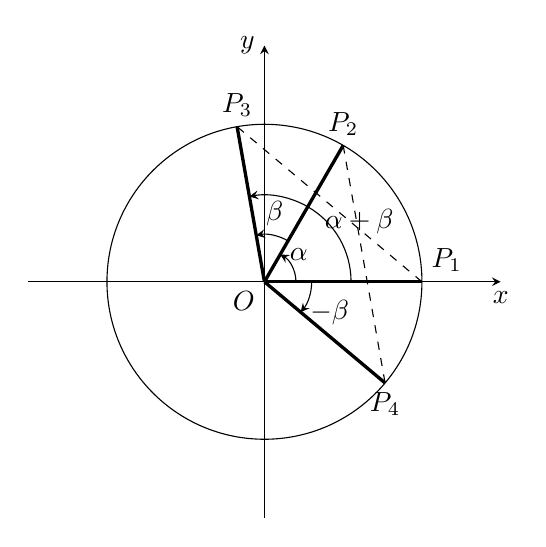
\begin{tikzpicture}[>=stealth]
  \draw[->](-3,0)--(3,0)node[below]{$x$};
\draw[->](0,-3,0)--(0,3)node[left]{$y$};
\draw[](0,0)node[below left]{$O$} circle (2);
\coordinate (P2) at (60:2);
\node at (P2)[above]{$P_2$};
\coordinate (P4) at (-40:2);
\node at (P4)[below]{$P_4$};
\coordinate (P3) at (100:2);
\node at (P3)[above]{$P_3$};
\coordinate (P1) at (0:2);
\node at (P1)[above right]{$P_1$};
\foreach \x in {1,2,3,4}
{
    \draw[very thick](P\x)--(0,0);
}
\draw[dashed](P2)--(P4);
\draw[dashed](P1)--(P3);

\draw[->](.4,0) arc (0:60:.4)node[right]{$\alpha$};
\draw[->](.6,0) arc (0:-40:.6)node[right]{$-\beta$};
\draw[->](60:.6) arc (60:100:.6)node[above right]{$\beta$};
\draw[->](1.1,0) arc (0:100:1.1);
\node at (50:1)[right]{$\alpha+\beta$};


\end{tikzpicture}
    \caption{}
\end{figure}

$\because\quad |P_1P_3|=|P_2P_4|$,由两点间距离公式得
\[[\cos(\alpha+\beta)-1]^2+\sin^2(\alpha+\beta)=[\cos\alpha-\cos(-\beta)]^2+[\sin\alpha-\sin(-\beta)]^2\]
展开,整理得:
\[2-2\cos(\alpha+\beta)=2-2(\cos\alpha\cos\beta-\sin\alpha\sin\beta)\]

$\therefore\quad \cos(\alpha+\beta)=\cos\alpha\cos\beta-\sin\alpha\sin\beta$\hfill(1)

这个公式对任意角$\alpha,\beta$都成立,再用$(-\beta)$代替$\beta$,就有
\[\cos(\alpha-\beta)=\cos\alpha\cos(-\beta)-\sin\alpha\sin(-\beta)\]
即
\begin{equation}
    \cos(\alpha-\beta)=\cos\alpha\cos\beta+\sin\alpha\sin\beta \tag{2}
\end{equation}

利用(1)(2)和诱导公式(七)可以推求$\sin(\alpha+\beta)$的表达式.

$\because\quad \sin(\alpha+\beta)=\cos\left[\frac{\pi}{2}-(\alpha+\beta)\right]$

而
\[\begin{split}
    \cos\left[\frac{\pi}{2}-(\alpha+\beta)\right]&=\cos\left[\left(\frac{\pi}{2}-\alpha\right)-\beta\right]
    \\
&=\cos\left(\frac{\pi}{2}-\alpha\right)\cos\beta+\sin\left(\frac{\pi}{2}-\alpha\right)\sin\beta\\
&=\sin\alpha\cos\beta+\cos\alpha\sin\beta
\end{split}\]

$\therefore\quad \sin(\alpha+\beta)=\sin\alpha\cos\beta+\cos\alpha\sin\beta$ \hfill(3)

再以$(-\beta)$代替$\beta$,又有
\[\sin(\alpha-\beta)=\sin\alpha\cos(-\beta)+\cos\alpha\sin(-\beta)=\sin\alpha\cos\beta-\cos\alpha\sin\beta\]
即
\begin{equation}
    \sin(\alpha-\beta)=\sin\alpha\cos\beta-\cos\alpha\sin\beta \tag{4}
\end{equation}

当$\cos(\alpha+\beta)\ne 0$时,利用(1)(3)又得:
\[\tan(\alpha+\beta)=\frac{\sin\alpha\cos\beta+\cos\alpha\sin\beta}{\cos\alpha\cos\beta-\sin\alpha\sin\beta}\]
当$\cos\alpha\cos\beta\ne 0$时,上式右边分子、分母同除以$\cos\alpha\cos\beta$,得:
\begin{equation}
    \tan(\alpha+\beta)=\frac{\tan\alpha+\tan\beta}{1-\tan\alpha\tan\beta}\tag{5}
\end{equation}
在(5)中,再以$(-\beta)$代替$\beta$,又有
\begin{equation}
    \tan(\alpha-\beta)=\frac{\tan\alpha-\tan\beta}{1+\tan\alpha\tan\beta}\tag{6}
\end{equation}

公式(1)、(3)、(5)实现了用单角$\alpha$、$\beta$的三角函数表示和角$(\alpha+\beta)$的三角函数的可能性,统称为\textbf{和角公式}。它不仅在计算上非常重要,而且是后续一系列三角公式推导的基础,因此,在理论上也十分重要。这组公式有的书又称为\textbf{三角函数的加法定理}。对它说明如下:

\begin{enumerate}
    \item 公式成立的条件:
    
    从推导过程可见,(1)、(3)对任意的$\alpha$、$\beta\in \R$都成立,(5)对任意的$\alpha,\beta,\alpha+\beta\in\R$,且$\ne \frac{\pi}{2}+k\pi\;(k\in\Z)$都成立,它们都是各自定义域上的恒等式。

\item 公式的功能:

    “从左往右”用,能把$(\alpha+\beta )$的函数,表成$\alpha$、$\beta$ 的函数;“从右往左”用,能把右边结构复杂的式子表示成$(\alpha+\beta )$的一个函数。
\item 公式的结构特征与记忆:
\begin{itemize}
    \item 公式(3)的右边是“正、余加余、正,角序是$\alpha,\beta$”;
    \item 公式(1)的右边是“余、余减正、正,角序也是$\alpha, \beta$”,
    \item 公式(5)是用$\tan\alpha$与$\tan\beta$ 的和与积表出了$\tan(\alpha+\beta)$.
\end{itemize}
    
    抓住了以上特征,就抓住了记忆和使用这些公式的线索。
\end{enumerate}    

    对于\textbf{差角公式}(2)、(4)、(6)可做类似地说明。

    有了和(差)角公式,借助过去已经熟悉的特殊角$30^{\circ}$、$45^{\circ}$、$60^{\circ}$的三角函数值,能求出由这三个角组成的各种和角或差角的函数值。

\begin{example}
    不查表,求$15^{\circ}$、$75^{\circ}$的正弦、余弦、正切值。
\end{example}

\begin{solution}
\[\begin{split}
\sin15^{\circ}=\sin(45^{\circ}-30^{\circ})&=\sin45^{\circ}\cos30^{\circ}-\cos45^{\circ}\sin30^{\circ}\\
&=\frac{\sqrt{2}}{2}\cdot \frac{\sqrt{3}}{2}-\frac{\sqrt{2}}{2}\cdot \frac{1}{2}=\frac{\sqrt{6}-\sqrt{2}}{4}
\end{split} \]
\[\begin{split}
    \cos15^{\circ}=\cos(45^{\circ}-30^{\circ})&=\cos45^{\circ}\cos30^{\circ}+\sin45^{\circ}\sin30^{\circ}\\
    &=\frac{\sqrt{2}}{2}\cdot \frac{\sqrt{3}}{2}+\frac{\sqrt{2}}{2}\cdot \frac{1}{2}=\frac{\sqrt{6}+\sqrt{2}}{4}
\end{split} \]
\[\begin{split}
    \tan15^{\circ}=\frac{\sin15^{\circ}}{\cos15^{\circ}}&=\frac{\sqrt{6}-\sqrt{2}}{4}\cdot \frac{4}{\sqrt{6}+\sqrt{2}}\\
    &=\frac{\sqrt{3}-1}{\sqrt{3}+1}=2-\sqrt{3}
\end{split} \]
利用诱导公式,得
\[\begin{split}
\sin75^{\circ}&=\cos15^{\circ}=\frac{\sqrt{6}+\sqrt{2}}{4}\\
\cos75^{\circ}&=\sin15^{\circ}=\frac{\sqrt{6}-\sqrt{2}}{4}\\
\tan75^{\circ}&=\cot15^{\circ}=\frac{1}{\tan15^{\circ}}=\frac{1}{2-\sqrt{3}}=2+\sqrt{3}
\end{split} \]
\end{solution}

\begin{example}
已知$\sin\alpha=\frac{2}{3}$,$\alpha\in\left(\frac{\pi}{2},\; \pi\right)$,$\cos\beta=-\frac{3}{4}$,$\beta\in\left(\pi,\;\frac{3\pi}{2}\right)$

求$\sin(\alpha+\beta)$、$\cos(\alpha-\beta)$和$\tan(\alpha+\beta)$
\end{example}

\begin{analyze}
由于$\sin(\alpha+\beta)$、$\cos(\alpha-\beta)$的展开式中有$\cos\alpha$、$\sin\beta$,为此应先算出$\cos\alpha$、$\sin\beta$.
\end{analyze}

\begin{solution}
由$\sin\alpha=\frac{2}{3}$,$\alpha\in\left(\frac{\pi}{2},\; \pi\right)$,得
\[\cos\alpha=-\sqrt{1-\sin^2\alpha}=-\sqrt{1-\left(\frac{2}{3}\right)^2}=-\frac{\sqrt{5}}{3}\]
又由于$\cos\beta=-\frac{3}{4}$,$\beta\in\left(\pi,\; \frac{3\pi}{2}\right)$,得
\[\sin\beta=-\sqrt{1-\cos^2\beta}=-\sqrt{1-\left(\frac{3}{4}\right)^2}=-\frac{\sqrt{7}}{4}\]

\[\begin{split}
    \therefore\quad \sin(\alpha+\beta)&=\sin\alpha\cos\beta+\cos\alpha\sin\beta\\
&=\frac{2}{3}\left(-\frac{3}{4}\right)+\left(-\frac{\sqrt{5}}{3}\right)\left(-\frac{\sqrt{7}}{4}\right)=\frac{-6+\sqrt{35}}{12}\\
\cos(\alpha-\beta)&=\cos\alpha\cos\beta+\sin\alpha\sin\beta\\
&=\left(-\frac{\sqrt{5}}{3}\right)\left(-\frac{3}{4}\right)+\frac{2}{3}\left(-\frac{\sqrt{7}}{4}\right)=\frac{3\sqrt{5}-2\sqrt{7}}{12}\\
\end{split}\]

又$\cos(\alpha+\beta)=\cos\alpha\cos\beta-\sin\alpha\sin\beta=\frac{3\sqrt{5}+2\sqrt{7}}{12}$

\[\begin{split}
\because\quad \tan(\alpha+\beta)=\frac{\sin(\alpha+\beta)}{\cos(\alpha+\beta)}&=\frac{\frac{-6+\sqrt{35}}{12}}{\frac{3\sqrt{5}+2\sqrt{7}}{12}}\\
&=\frac{-6+\sqrt{35}}{3\sqrt{5}+2\sqrt{7}}=\frac{-32\sqrt{5}+27\sqrt{7}}{17}
\end{split}\]
\end{solution}

\begin{thm}
    {思考题}
\begin{enumerate}[(1)]
\item 在此例中,你还能想出算$\tan(\alpha+\beta)$的办法吗?
\item 若知道$\alpha$、$\beta$的各自任何一种角函数值,那么
$(\alpha\pm\beta)$的任何一种角函数值是否都能用上述方法求得?说明理由。
\end{enumerate}
\end{thm}

\section*{习题一}
\begin{center}
    \bfseries A
\end{center}

\begin{enumerate}
    \item 不查表,求下列各式的值。
\begin{multicols}{2}
\begin{enumerate}[(1)]
    \item $105^{\circ}$的正弦、余弦、正切
    \item  $\cos 165^{\circ }$
    \item $\sin \left ( - \frac 5{12}\pi \right ) $
    \item $\sin \left ( - \frac {65\pi }{12}\right ) $
\end{enumerate}    
\end{multicols}
\item 已知 $\sin\alpha = \frac {15}{17}$, $\alpha \in \left ( \frac \pi 2, \;\pi \right )$, 
    求$\sin\left(\frac\pi{3}+\alpha\right)$及$\cos\left(\frac\pi3-\alpha\right)$.
\item    已知 $\cos \theta = - \frac 5{13}$, $\theta \in \left (\pi , \; \frac {3}{2}\pi \right )$, 
    求$\sin\left(\theta-\frac\pi6\right)$及$\cos\left(\theta+\frac\pi6\right)$.
\item $\sin \alpha = \frac 23$, $\cos \beta = - \frac 34$, 且$\alpha$、 $\beta$ 都是第I象限角,求 $\sin(\alpha-\beta)$及$\cos(\alpha-\beta)$
\item \begin{enumerate}[(1)]
\item 已知$\tan x=\frac{1}{4}$,$\tan y=-3$, 求$\tan(x+y)$;
\item 已知$\tan \alpha = 2k+ 1$, $\tan\beta=2k-1$,求$\cot(\alpha-\beta)$.
\end{enumerate}

\item 已知$\cos \theta = - \frac {12}{13}$, $\theta \in \left(\pi,\; \frac{3}{2}\pi\right)$, 求$\sin\left(\theta-\frac{\pi}{4}\right)$、$\cos\left(\theta-\frac{\pi}{4}\right)$和$\tan\left(\theta-\frac{\pi}{4}\right)$.
\item 化简:
\begin{multicols}{2}
\begin{enumerate}[(1)]
    \item $\sin58^{\circ}\cos37^{\circ}-\cos 58^{\circ}\sin37^{\circ}$
    \item $\cos24^{\circ}\cos69^{\circ}-\sin24^{\circ}\sin69^{\circ}$
    \item $\cos12^{\circ}\cos28^{\circ}+\sin12^{\circ}\sin28^{\circ}$
    \item $\sin70^{\circ}\cos25^{\circ}-\sin20^{\circ}\sin25^{\circ}$
\end{enumerate}    
\end{multicols}

\end{enumerate}

\begin{center}
    \bfseries B
\end{center}

\begin{enumerate}\setcounter{enumi}{7}
    \item 参照下图,当$\alpha$、$\beta$都为正锐角时,利用三角形的面积公式推出$\sin(\alpha+\beta)$的公式
\begin{figure}[htp]
    \centering
\begin{tikzpicture}[>=stealth]
\tkzDefPoints{0/0/O, 4/0/C, 4/3/A, 4/-2/B}
\draw[very thick](O)--node[above]{$a$}(A)--(B)--node[below]{$b$}(O);
\draw[very thick](O)--(C);
\tkzMarkRightAngle(O,C,A)
\draw(O)--node[above]{$a\cos\alpha$}(C);
\draw(O)--node[below]{$b\cos\beta$}(C);
\draw(A)--node[right]{$a\sin\alpha$}(C);
\draw(B)--node[right]{$b\sin\beta$}(C);
\tkzMarkAngle[mark=none, size=.7cm](C,O,A)
\tkzMarkAngle[mark=none, arc=ll, size=.8cm](B,O,C)
\tkzLabelAngle(C,O,A){$\alpha$}
\tkzLabelAngle(B,O,C){$\beta$}

\end{tikzpicture}
    \caption*{(第8题)}
\end{figure}

\item 已知$\tan\alpha=\frac{1}{3}$,$\tan\beta=-2$,
\begin{enumerate}[(1)]
    \item 求$\cot(\alpha-\beta)$
    \item 求$\tan(\alpha+\beta)$
    \item 求$\sin^2(\alpha+\beta)-\sin(\alpha+\beta)\cos(\alpha+\beta)-\cos^2(\alpha+\beta)$
\end{enumerate}

\item 设$\tan\alpha$, $\tan\beta$是一元二次方程$ax^2+bx+c=0\; (b\ne 0)$的两个根,求$\cot(\alpha+\beta)$的值.
\end{enumerate}

\begin{example}
 利用和角公式证明以下两组诱导公式:  
\[\text{(八)}\begin{cases}
    \sin\left(\frac{3\pi}{2}+\alpha\right)=-\cos\alpha\\
    \cos\left(\frac{3\pi}{2}+\alpha\right)=\sin\alpha\\
    \tan\left(\frac{3\pi}{2}+\alpha\right)=-\cot\alpha\\
    \cot\left(\frac{3\pi}{2}+\alpha\right)=-\tan\alpha\\
\end{cases}\quad \text{(九)}\begin{cases}
    \sin\left(\frac{3\pi}{2}-\alpha\right)=\cos\alpha\\
    \cos\left(\frac{3\pi}{2}-\alpha\right)=-\sin\alpha\\
    \tan\left(\frac{3\pi}{2}-\alpha\right)=\cot\alpha\\
    \cot\left(\frac{3\pi}{2}-\alpha\right)=\tan\alpha\\
\end{cases}\]
 (请读者完成)
\end{example}

现在对诱导公式(六)、(七)、(八)、(九)做一些说明:
\begin{enumerate}
\item 公式左边的角为$\left(\frac{\pi}{2}\pm \alpha\right)$和$\left(\frac{3\pi}{2}\pm \alpha\right)$,其中$\frac{\pi}{2}$与$\frac{3\pi}{2}$都可以写成$\frac{\pi}{2}\cdot n\; (n=1,3)$,是直角的奇数倍,其终边都落在$y$轴上。这与1.4节中的角$(\pi\pm\alpha)$、$(2\pi-\alpha)$、$-\alpha$、$2k\pi+\alpha\; (k\in\Z)$不同,那里的$\pi$、$2\pi$、0、$2k\pi$都可以写成$\frac{\pi}{2}\cdot n\; (n=0,2,4,\ldots)$是直角的偶数倍,其终边都落在$x$轴上。
\item 公式右边的函数都是左边函数的余名函数。这也与1.4节的情况不同,那里左、右两边是同名函数。
\item 公式右边的符号与$\alpha$为锐角时左边函数值的符号一致,这一点与1.4节的情况相同。因此,也可以说成是“符号看象限”。
\end{enumerate}

基于上述分析,前后九组诱导公式的左边可以统一写成
$f\left(\frac{\pi}{2}\cdot n\pm \alpha\right)$,
当$n$为奇数时,右边变为余名函数;当$n$为偶数时,右边仍为同名函数,符号一律取$\alpha$为锐角时,左边函数值的符号,为便于记忆,这可简述为“奇变偶不变,符号看象限”。

诱导公式的主要功能是化简。能把一个任意角的函数,通过“去负”、“去周”、“化锐角”的方法,最后化成锐角的三角函数。这对函数的研究与计算无疑会带来很大的方便。但是诱导公式的其他功能也不容忽视,如当n为奇数时,“从右往左”用它,可以把一个函数变为余名函数。例如,
\[\begin{split}
\sin\alpha=\cos\left(\frac{\pi}{2}-\alpha\right),&\qquad 
\cos\alpha=\sin\left(\frac{\pi}{2}-\alpha\right)\\
\tan\alpha=\cot\left(\frac{\pi}{2}-\alpha\right),&\qquad 
\cot\alpha=\tan\left(\frac{\pi}{2}-\alpha\right)
\end{split}\]
这种改变函数名称的方法无论在计算上还是在函数性质的研究上,都是有用的。

\noindent
\begin{minipage}{.55\textwidth}
\begin{example}
把$\cos\frac{4\pi}{5}$化为:
\begin{enumerate}[(1)]
    \item 锐角的同名函数;
    \item 锐角的余名函数。
\end{enumerate}
\end{example}

\begin{solution}
\begin{enumerate}[(1)]
    \item $\cos\frac{4\pi}{5}=\cos\left(\pi-\frac{\pi}{5}\right)=-\cos\frac{\pi}{5}$
    
    (图2.3)
    \item $\cos\frac{4\pi}{5}=\sin\left(\frac{\pi}{2}-\frac{4\pi}{5}\right)=-\sin\frac{3\pi}{10}$
    
或
\[\cos\frac{4\pi}{5}=\cos\left(\frac{\pi}{2}+\frac{3\pi}{10}\right)=-\sin\frac{3\pi}{10}\]    
\end{enumerate}
\end{solution}    
\end{minipage}\hfill
\begin{minipage}{.35\textwidth}
\centering
\begin{tikzpicture}[>=stealth]
\draw[->](-2.15,0)--(2.15,0)node[below]{$x$};
\draw[->](0,-2.15)--(0,2.25)node[left]{$y$};
\draw(0,0)node[below left]{$O$} circle(1.5);
\draw[very thick](0,0)--(144:1.5);
\draw[thick,->](.5,0) arc (0:144:.5);
\node at (72:.5)[above right]{$\tfrac{4\pi}{5}$};
\end{tikzpicture}
\captionof{figure}{}
\end{minipage}

\begin{example}
    不查表,求$\sin113^{\circ}\cos22^{\circ}+\sin203^{\circ}\sin155^{\circ}$的值。
\end{example}

\begin{analyze}
由所给式子的结构,容易想到应“从右往左”用和(差)角公式。但形式上$\alpha$、$\beta$及函数名称都不规范,须用诱导公式对后一项进行适当变形.
\end{analyze}

\begin{solution}
\[\begin{split}
\because\quad \sin203^{\circ}&=\sin(90^{\circ}+113^{\circ})=\cos113^{\circ}\\
\sin 158^{\circ}&=\sin(180^{\circ}-22^{\circ})=\sin 22^{\circ}
\end{split}\]

$\therefore\quad \text{原式}=\sin113^{\circ}\cos22^{\circ}+\cos113^{\circ}\sin22^{\circ}=\sin135^{\circ}=\frac{\sqrt{2}}{2}$
\end{solution}

\begin{example}
化简下列各式:
\begin{multicols}{2}
\begin{enumerate}[(1)]
    \item $\frac{1}{2}\cos x-\frac{\sqrt{3}}{2}\sin x$
    \item $\sqrt{3}\sin x+\cos x$
    \item $\sin x-\cos x$
\end{enumerate}
\end{multicols}
\end{example}

\begin{solution}
\begin{enumerate}[(1)]
    \item $\text{原式}=\sin\frac{\pi}{6}\cos x-\cos\frac{\pi}{6}\sin x=\sin\left(\frac{\pi}{6}-x\right)$
    \item $\text{原式}=2\left(\frac{\sqrt{3}}{2}\sin x+\frac{1}{2}\cos x\right)=2\left(\sin x\cos\frac{\pi}{6}+\cos x\sin\frac{\pi}{6}\right)=2\sin\left(x+\frac{\pi}{6}\right)$
    \item $\text{原式}=\sqrt{2}\left(\sin x\cdot \frac{\sqrt{2}}{2}-\cos x\cdot \frac{\sqrt{2}}{2}\right)=\sqrt{2}\left(\sin x\cdot \cos\frac{\pi}{4}-\cos x\cdot \sin\frac{\pi}{4}\right)=\sqrt{2}\sin\left(x-\frac{\pi}{4}\right)$
\end{enumerate}
\end{solution}

\begin{example}
计算$\frac{1+\tan15^{\circ}}{1-\cot75^{\circ}}$
\end{example}

\begin{analyze}
    利用$1=\tan45^{\circ}$,可把原式改写成
$\frac{\tan45^{\circ}+\tan15^{\circ}}{1-\tan45^{\circ}\cdot \cot75^{\circ}}$,从而,可以“从右往左”运用和角公式.
\end{analyze}

\begin{solution}
$\because\quad 1=\tan 45^{\circ},\quad \cot75^{\circ}=\tan 15^{\circ}$

$\therefore\quad \text{原式}=\frac{\tan45^{\circ}+\tan15^{\circ}}{1-\tan45^{\circ} \tan15^{\circ}}=\tan(45^{\circ}+15^{\circ})=\sqrt{3}$
\end{solution}

\section*{习题二}
\begin{center}
    \bfseries A
\end{center}

\begin{enumerate}
    \item 把$\sin\frac{11\pi}{8}$化为
\begin{multicols}{3}
\begin{enumerate}[(1)]
    \item 锐角的同名函数;
    \item 锐角的余名函数;
    \item $0\sim \frac{\pi}{4}$的三角函数.
\end{enumerate}
\end{multicols}

\item 化简:
\begin{enumerate}[(1)]
    \item $\cos80^{\circ}\cos20^{\circ}+\sin80^{\circ}\sin20^{\circ}$
    \item $\cos^{2}15^{\circ}-\sin^{2}15^{\circ}$
    \item $\sin14^{\circ}\cos16^{\circ}+\sin76^{\circ}\cos74^{\circ}$ 
    \item $\sin21^{\circ}\cos81^{\circ}-\sin69^{\circ}\cos9^{\circ}$ 
    \item $\sin\left(\alpha-\beta\right)\cos\beta+\cos\left(\alpha-\beta\right)\sin\beta$ 
    \item $\cos\left(\alpha+\beta\right)\cos\beta+\sin\left(\alpha+\beta\right)\sin\beta$ 
    \item $\cos\left(36^{\circ}+x\right)\cos\left(54^{\circ}-x\right)-\sin(36^{\circ}+x)\sin(54^{\circ}-x)$
    \item $\sin\left(70^{\circ}+\alpha\right)\cos\left(10^{\circ}+\alpha\right)-\cos\left(70^{\circ}+\alpha\right)\sin\left(170^{\circ}-\alpha\right)$
\end{enumerate}

\item 化简:
\begin{enumerate}[(1)]
    \item $\sin347^{\circ}\cos148^{\circ}+\sin77^{\circ}\cos58^{\circ}$
    \item $\sin164^{\circ}\sin224^{\circ}+\sin254^{\circ}\sin314^{\circ}$
    \item $\cos(\alpha-\beta)\cos(\beta-\gamma)-\sin(\alpha-\beta)\sin(\beta-\gamma)$
    \item $\cos(\theta-\varphi)\cos\varphi+\sin(\theta-\varphi)\sin\varphi$
\end{enumerate}

\item 化简:
\begin{multicols}{2}
\begin{enumerate}[(1)]
    \item $\frac{\sqrt{3}}{2}\cos x-\frac{3}{2}\sin x$
    \item $\sqrt{2}(\sin x-\cos x)$
    \item $\sqrt{3}\sin x+\cos x$
\end{enumerate}
\end{multicols}

\item 在$\triangle ABC$中:
\begin{enumerate}[(1)]
    \item 已知$\cos A=\frac{4}{5}$,$\cos B=\frac{12}{13}$,求$\cos C$
    \item 已知$\sin A=\frac{3}{5}$,$\cos B=\frac{5}{13}$,求$\cos C$
\end{enumerate}
(提示:应能看出$B$都是锐角,那么$A$能是钝角吗?)

\item 化简:
\begin{multicols}{2}
\begin{enumerate}[(1)]
    \item $\frac{\tan53^{\circ}-\tan 23^{\circ}}{1+\tan53^{\circ}\cot67^{\circ}}$
    \item $\frac{\tan2\theta-\tan\theta}{1+\tan2\theta\tan\theta}$
    \item $\frac{1+\tan15^{\circ}}{1+\cot 75^{\circ}}$
    \item $\frac{1+\tan\theta}{1-\tan\theta}$
\end{enumerate}
\end{multicols}

\item 求证:
\begin{enumerate}[(1)]
    \item $\tan(x+y)\cdot \tan(x-y)=\frac{\tan^2 x-\tan^2 y}{1-\tan^2 x\tan^2 y}$
    \item $\cot\left(\frac{\pi}{4}-\theta\right)=\frac{1+\tan\theta}{1-\tan\theta}$
    \item $\frac{\tan x+\tan y}{\tan x-\tan y}=\frac{\sin(x+y)}{\sin(x-y)}$
\end{enumerate}
\end{enumerate}

\begin{center}
    \bfseries B
\end{center}

\begin{enumerate}\setcounter{enumi}{7}
    \item 用$\cot\alpha$、$\cot\beta$表示$\cot(\alpha\pm\beta)$,并求$\frac{1-\cot15^{\circ}}{1+\cot15^{\circ}}$的值.
\item 已知$\cos(\alpha-\beta)=-\frac{4}{5}$,$\cos(\alpha+\beta)=\frac{4}{5}$,且$(\alpha-\beta)\in\left(\frac{\pi}{2},\pi\right)$,$(\alpha+\beta)\in\left(\frac{3\pi}{2},2\pi\right)$

求$\cos2\alpha$、$\cos2\beta$ 
[提示:$2\alpha=(\alpha-\beta)+(\alpha+\beta)$]

\item 已知$\cos\alpha=\frac{1}{7}$,$\cos(\alpha+\beta)=-\frac{11}{14}$,且$\alpha,\beta\in\left(0,\frac{\pi}{2}\right)$,求$\cos\beta$.

\item 已知$\alpha,\beta$为锐角,$\sin\alpha=\frac{3}{5}$,$\tan(\alpha-\beta)=-\frac{1}{3}$,求$\cos\beta$.

\item 已知$\sin\alpha-\sin\beta=-\frac{1}{3}$,$\cos\alpha-\cos\beta=\frac{1}{2}$,求$\cos(\alpha-\beta)$的值.

[提示:思考$\cos(\alpha-\beta)$展开式的结构怎样由已知直接得到]
\end{enumerate}

\begin{center}
    \bfseries C
\end{center}
\begin{enumerate}\setcounter{enumi}{12}
    \item 推求以单角$\alpha,\beta,\gamma$的函数表达$\sin(\alpha+\beta+\gamma)$与$\cos(\alpha+\beta+\gamma)$的公式.
\end{enumerate}

现在进一步谈谈灵活使用公式$\tan(\alpha+\beta)=\frac{\tan\alpha+\tan\beta}{1-\tan\alpha\tan\beta}$
的问题。前面讲过,这个公式的结构特征是用$\tan\alpha$、$\tan\beta$的\textbf{和与积}表示出了$\tan(\alpha+\beta)$. 因此,所给问题中,若出现了$\tan\alpha$、$\tan\beta$的和与积,你就应“联想”这个公式。

\begin{example}
   求证:$\tan20^{\circ}+\tan40^{\circ}+\sqrt{3}\tan 20^{\circ}\cdot \tan40^{\circ}=\sqrt{3}$ 
\end{example}

\begin{solution}
由$\frac{\tan20^{\circ}+\tan40^{\circ}}{1-\tan20^{\circ}\tan40^{\circ}}=\tan(20^{\circ}+40^{\circ})=\sqrt{3}$,得
\[\tan20^{\circ}+\tan40^{\circ}=\sqrt{3}\left(1-\tan20^{\circ}\tan40^{\circ}\right)\]

$\therefore\quad \tan20^{\circ}+\tan40^{\circ}+\sqrt{3}\tan 20^{\circ} \tan40^{\circ}=\sqrt{3}$
\end{solution}

\begin{example}
若$A+B=225^{\circ}$,求证:
\begin{equation}
    \frac{\cot A}{1+\cot A}\cdot \frac{\cot B}{1+\cot B}=\frac{1}{2}\tag{1}
\end{equation}
\end{example}

\begin{proof}
\begin{align}
\text{左}&=\frac{1}{1+\tan A}\cdot \frac{1}{1+\tan B}\nonumber\\
&=\frac{1}{\tan A\tan B+(\tan A+\tan B)+1}\tag{2}
\end{align}
(注意,这里出现了“正切的和与积”!)

由$\frac{\tan A+\tan B}{1-\tan A\tan B}=\tan(A+B)=\tan 225^{\circ}=1$,得
\begin{equation}
    \tan A+\tan B=1+\tan A\tan B\tag{3}
\end{equation}
(3)代入(2),得
\[\text{左边}=\frac{1}{\tan A\tan B+(1-\tan A\tan B)+1}=\frac{1}{2}\Rightarrow (1)\text{成立}\]
  \end{proof}  

\section*{习题三}  
\begin{center}
    \bfseries B
\end{center}
    
\begin{enumerate}
    \item 求证:$ \tan 95^\circ-\tan 35^\circ-\sqrt{3}=\sqrt{3} \tan 95^\circ\cdot\tan 35^\circ$,
    \item 已知$\tan \alpha$、$\tan \beta$是方程$x^2+6x+7=0$的两个根,
\begin{enumerate}[(1)]
    \item 求证:$\sin(\alpha+\beta)=\cos(\alpha+\beta)$
\item 求$\sin(\alpha+\beta)\cos(\alpha+\beta)+8\cos^2(\alpha+\beta)$的值
\end{enumerate}
\item 若$\alpha+\beta+\gamma=n\pi\; \left(n\in \Z\right)$, 求证:
$$\tan\alpha+\tan \beta+\tan \gamma=\tan \alpha\tan \beta\tan \gamma$$
\item 求证:$$\tan (x-y)+\tan (y-z)+\tan (z-x)=\tan (x-y)\tan (y-z)\tan (z-x)$$
\item $\theta=15^{\circ}$,求$ \tan \frac\theta2+\tan \frac\theta2\tan \frac{5\theta}{2}+\tan \frac{5\theta}{2}$的值。
\end{enumerate}

\begin{center}
    \bfseries C
\end{center}

\begin{enumerate}\setcounter{enumi}{5}
    \item 化简:$$\tan2A \tan(30^{\circ}-A)+ \tan2A \tan(60^{\circ}-A) +\tan\left(60^{\circ}-A\right)\tan \left(30^{\circ}-A\right)$$
\end{enumerate}

\section{倍角的正弦、余弦、正切}
在和角公式中,以$\alpha$代替$\beta$,得到\textbf{二倍角公式}:
\begin{align}
\sin2\alpha&=2\sin\alpha\cos\alpha \nonumber\\
\cos2\alpha&=\cos^2\alpha-\sin^2\alpha\nonumber\\
&=2\cos^2\alpha-1=1-2\sin^2\alpha \tag{$\sin^2\alpha=1-\cos^2\alpha$}\\
\tan2\alpha&=\frac{2\tan\alpha}{1-\tan^2\alpha}    \nonumber
\end{align}

在2.2节中关于和角公式的说明,这里也完全适用。

\begin{example}
已知$\sin\alpha=\frac{5}{13}$,$\alpha\in\left(\frac{\pi}{2},\pi\right)$,求$\sin2\alpha$, $\cos2\alpha$, $\tan2\alpha$. 
\end{example}

\begin{solution}
    由$\sin\alpha=\frac{5}{13}$,$\alpha\in\left(\frac{\pi}{2},\pi\right)$,得:
\[\cos2\alpha=-\sqrt{1-\sin^2\alpha}=-\sqrt{1-\left(\frac{5}{13}\right)^2}=-\frac{12}{13}\]

\[\begin{split}
\therefore\quad \sin2\alpha&=2\sin\alpha\cos\alpha=2\x\frac{5}{13}\x\left(-\frac{12}{13}\right)=-\frac{120}{169}    \\
\cos2\alpha&=1-2\sin^2\alpha =1-2\x\left(\frac{15}{13}\right)^2=\frac{119}{169}\\
\tan2\alpha&=\frac{\sin2\alpha}{\cos2\alpha}=\frac{-\frac{120}{169}}{\frac{119}{169}}=-\frac{120}{119}
\end{split}\]
\end{solution}


\begin{example}
\begin{enumerate}[(1)]
    \item 用$\sin\theta$表示$\sin3\theta$;
    \item 用$\cos\theta$表示$\cos3\theta$.
\end{enumerate}
\end{example}

\begin{solution}
\[\begin{split}
    (1)\quad \sin3\theta =\sin(2\theta+\theta)&=\sin2\theta\cos\theta+\cos2\theta\sin\theta\\
&=2\sin\theta\cos^2\theta+(1-2\sin^2\theta)\sin\theta\\
&=2\sin\theta(1-\sin^2\theta)+\sin\theta-2\sin^3\theta\\&=3\sin\theta-4\sin^3\theta
    \end{split}\]

$\therefore\quad \sin3\theta =3\sin\theta-4\sin^3\theta$ \hfill(1)   

\[\begin{split}
(2)\quad \cos3\theta =\cos(2\theta+\theta)&=\cos2\theta\cos\theta-\sin2\theta\sin\theta\\
&=(2\cos^2\theta-1)\cos\theta-2\sin^2\theta\cos\theta\\
&=2\cos^3\theta-\cos\theta-2(1-\cos^2\theta)\cos\theta\\&=4\cos^3\theta-3\cos\theta
    \end{split}\]

$\therefore\quad \cos3\theta =4\cos^3\theta-3\cos\theta$\hfill(2)
\end{solution}

\begin{rmk}
    (1)(2)也可写成降幂形式:
\[\begin{split}
    4\sin^3\theta &=3\sin\theta-\sin3\theta\\
    4\cos^3\theta &=3\cos\theta+\cos3\theta\\
\end{split}\]
\end{rmk}

\begin{example}
求证:
\[[\sin\theta(1+\sin\theta)+\cos\theta(1+\cos\theta)]\x [\sin\theta(1-\sin\theta)+\cos\theta(1-\cos\theta)]=\sin2\theta\]
\end{example}

\begin{analyze}
差异主要在运算上,应从左到右,由繁化简.
\end{analyze}


\begin{proof}
\[\begin{split}
\text{左边}&=(\sin\theta+\sin^2\theta+\cos\theta+\cos^2\theta)(\sin\theta-\sin^2\theta+\cos\theta-\cos^2\theta)\\
&=(\sin\theta+\cos\theta+1)(\sin\theta+\cos\theta-1)\\
&=(\sin\theta+\cos\theta)^2-1 =2\sin\theta\cos\theta+1-1=\sin2\theta
\end{split}\]

$\therefore\quad $原式成立.
\end{proof}



\begin{example}
化简:$\sin50^{\circ}\left(1+\sqrt{3}\tan 10^{\circ}\right)$
\end{example}

\begin{analyze}
    从角入手,用和(差)角公式,很繁. 考虑到特殊值$\sqrt{3}$,有下面两种方法。
\end{analyze}



\begin{solution}
\textbf{解法1:}
\[\begin{split}
    1+\sqrt{3}\tan 10^{\circ}&=1+\frac{\sqrt{3}\sin10^{\circ}}{\cos 10^{\circ}}=\frac{\cos10^{\circ}+\sqrt{3}\sin 10^{\circ}}{\cos 10^{\circ}}\\
&=\frac{2\left(\frac{1}{2}\cos 10^{\circ}+\frac{\sqrt{3}}{2}\sin 10^{\circ}\right)}{\cos 10^{\circ}}\\
&=\frac{2(\sin30^{\circ}\cos 10^{\circ}+\cos 30^{\circ}\sin 10^{\circ})}{\cos 10^{\circ}}=\frac{2\sin 40^{\circ}}{\cos 10^{\circ}}
\end{split}\]
\[ \therefore\quad \text{原式}=\sin50^{\circ}\cdot \frac{2\sin40^{\circ}}{\cos 10^{\circ}}=\frac{2\sin 40^{\circ}\cos 10^{\circ}}{\cos 10^{\circ}}=\frac{\sin80^{\circ}}{\cos 10^{\circ}}=\frac{\cos 10^{\circ}}{\cos 10^{\circ}}=1\]

\textbf{解法2:}
\[1+\sqrt{3}\tan10^{\circ}=1+\tan 60^{\circ}\tan 10^{\circ}=\frac{\tan 60^{\circ}-\tan 10^{\circ}}{\tan 50^{\circ}}\]
(以下留给读者完成)
\end{solution}

应该明确:对于“二倍角”应该有广义的理解,如$8\alpha$是$4\alpha$的二倍角,因此有:
\[\sin8\alpha=2\sin4\alpha\cos4\alpha,\; \ldots\]
又如,$a=2\cdot \frac{\alpha}{2},\; \frac{\alpha}{2}=2\cdot \frac{\alpha}{4},\; \ldots, \frac{\alpha}{2^n}=2\cdot \frac{\alpha}{2^{n+1}}$
\[\begin{split}
    \therefore\quad \sin\frac{\alpha}{2^n}&=2\sin\frac{\alpha}{2^{n+1}}\cos\frac{\alpha}{2^{n+1}}\qquad
    \cos\frac{\alpha}{2^{n}}=\cos^2\frac{\alpha}{2^{n+1}}-\sin^2\frac{\alpha}{2^{n+1}}\\
    \tan\frac{\alpha}{2^{n}}&=\frac{2\tan\frac{\alpha}{2^{n+1}}}{1-\tan^2\frac{\alpha}{2^{n+1}}}\quad (n\in\Z)
\end{split}\]

此外,二倍角公式的下列变形\footnote{要注意分析这些公式中等号两边式子的结构特征(角、函数、运算).这对何时使用它们是很有用的. 公式(1)、(2)、(3)称为\textbf{降幂式}.},今后也是有用的:
\begin{center}
\begin{tabular}{c|c}
\hline
    二倍角公式  & 变形\\
\hline
$\sin2\alpha=2\sin\alpha\cos\alpha$ & $\cos\alpha=\frac{\sin2\alpha}{2\sin\alpha}$\\[1.5ex]
$\cos2\alpha=\cos^2\alpha-\sin^2\alpha$&$\cos2\alpha=(\cos\alpha+\sin\alpha)(\cos\alpha-\sin\alpha)$\\[1.5ex]
$\cos2\alpha=2\cos^2\alpha-1$ & $\cos^2\alpha=\frac{1+\cos2\alpha}{2}$\hfill(1)\\[1.5ex]
$\cos2\alpha=1-2\sin^2\alpha$ & $\sin^2\alpha=\frac{1-\cos2\alpha}{2}$\hfill(2)\\[1.5ex]
$\tan2\alpha=\frac{2\tan\alpha}{1-\tan^2\alpha}$&$\tan^2\alpha=\frac{1-\cos2\alpha}{1+\cos2\alpha}$\hfill(3)\\[1.5ex]
\hline
\end{tabular}
\end{center}

\section*{习题四}
\begin{center}
    \bfseries A
\end{center}

\begin{enumerate}
    \item 不查表,求下列各式的值。
\begin{multicols}{2}
\begin{enumerate}[(1)]
    \item $2\sin67^{\circ}30'\; \cos67^{\circ}30'$
    \item $\cos^2\frac{\pi}{8}-\sin^2\frac{\pi}{8}$
    \item $2\cos^2\frac{\pi}{12}-1$
    \item $1-2\sin^2 75^{\circ}$
    \item $\frac{2\tan 22.5^{\circ}}{1-\tan^2 22.5^{\circ}}$
    \item $\sin 15^{\circ}\cos 15^{\circ}$
    \item $1-2\sin^2 750^{\circ}$
    \item $\frac{2\tan150^{\circ}}{1-\tan^2 150^{\circ}}$
    \item $\sin^2\frac{\pi}{16}-\cos^2\frac{\pi}{16}$
    \item $\frac{\tan\frac{5\pi}{24}}{1-\tan^2\frac{5\pi}{24}}$
\end{enumerate}
\end{multicols}

\item 化简:
\begin{multicols}{2}
\begin{enumerate}[(1)]
    \item $(\sin\alpha-\cos\alpha)^2$
    \item $\sin\frac{\theta}{2}\cos\frac{\theta}{2}$
    \item $\cos^4\varphi -\sin^4\varphi$
    \item $\frac{1}{1-\tan\theta}-\frac{1}{1+\tan\theta}$
\end{enumerate}
\end{multicols}

\item 已知$\sin\alpha=0.3$,$\alpha\in\left(0,\frac{\pi}{2}\right)$,求$\sin2\alpha$, $\cos2\alpha$.
\item 已知$\cos\alpha=-\frac{12}{13}$,$\alpha\in\left(\frac{\pi}{2},\pi\right)$,求$\cos2\alpha$、$\sin2\alpha$、$\tan2\alpha$、$\cot2\alpha$.

\item 已知$\tan\alpha=\frac{1}{2}$,求$\tan2\alpha$、$\cot2\alpha$.

\item 推出由$\tan\alpha$表示$\tan3\alpha$的公式.
\item 化简:
\begin{multicols}{2}
\begin{enumerate}[(1)]
    \item $\frac{1}{\sin10^{\circ}}-\frac{\sqrt{3}}{\cos10^{\circ}}$
    \item $\frac{\sqrt{3}}{4\sin 20^{\circ}}-\frac{1}{4\sin 70^{\circ}}$
    \item $\frac{1}{\cos^2 280^{\circ}}-\frac{3}{\sin^2 280^{\circ}}$
\end{enumerate}
\end{multicols}
    
\item 已知$\cos\alpha=-\frac{4}{5}$,求$\sin2\alpha$、$\cos2\alpha$(注意与题4对比).
\item 求证:$\frac{\sin\left(\frac{\pi}{4}+x\right)}{\sin\left(\frac{\pi}{4}-x\right)}+\frac{\cos\left(\frac{\pi}{4}+x\right)}{\cos\left(\frac{\pi}{4}-x\right)}=2\sec 2x$

\end{enumerate}

\begin{center}
    \bfseries B
\end{center}
\begin{enumerate}\setcounter{enumi}{9}
    \item 化简:$\frac{2\cos^2\alpha-1}{2\tan\left(\frac{\pi}{4}-\alpha\right)\cdot \sin^2 \left(\frac{\pi}{4}+\alpha\right)}$
(注意:分母上的角互余)

\item 求证:$\tan70^{\circ}-\frac{1}{\cos 10^{\circ}}=\sqrt{3}$
\item 不查表,利用$\tan15^{\circ}=2-\sqrt{3}$,求$\tan 7.5^{\circ}$的值.

\end{enumerate}


\section{半角的正弦、余弦、正切}
在上节的降幂式中,以$\frac{\alpha}{2}$代替$\alpha$,得
\[\begin{cases}
\sin^2\frac{\alpha}{2}=\frac{1-\cos\alpha}{2}\\[1.5ex]
\cos^2\frac{\alpha}{2}=\frac{1+\cos\alpha}{2}\\[1.5ex]
\tan^2\frac{\alpha}{2}=\frac{1-\cos\alpha}{1+\cos\alpha}
\end{cases}\xrightarrow[]{\text{开平方}}\begin{cases}
    \sin\frac{\alpha}{2}=\pm\sqrt{\frac{1-\cos\alpha}{2}}&(1)\\[1.5ex]
\cos\frac{\alpha}{2}=\pm\sqrt{\frac{1+\cos\alpha}{2}}&(2)\\[1.5ex]
\tan\frac{\alpha}{2}=\pm\sqrt{\frac{1-\cos\alpha}{1+\cos\alpha}}&(3)
\end{cases}\]

(1)、(2)、(3)称为\textbf{半角公式}. 这三个公式中,右边根号前的符号,由$\frac{\alpha}{2}$所在的象限确定。因此,在使用半角公式时,判断$\frac{\alpha}{2}$所在的象限是首要的步骤。

$\tan\frac{\alpha}{2}$
还可以用不带根号的式子表示:
\[\tan\frac{\alpha}{2}=\frac{\sin\frac{\alpha}{2}}{\cos\frac{\alpha}{2}}=\frac{\sin\frac{\alpha}{2}\cdot 2\cos \frac{\alpha}{2}}{\cos \frac{\alpha}{2}\cdot 2\cos\frac{\alpha}{2}}=\frac{\sin\alpha}{1+\cos\alpha}\]
或
\[\tan\frac{\alpha}{2}=\frac{\sin\frac{\alpha}{2}}{\cos\frac{\alpha}{2}}=\frac{\sin\frac{\alpha}{2}\cdot 2\sin \frac{\alpha}{2}}{\cos \frac{\alpha}{2}\cdot 2\sin\frac{\alpha}{2}}=\frac{1-\cos\alpha}{\sin\alpha}\]
即
\begin{equation}
\tan\frac{\alpha}{2}=\frac{\sin\alpha}{1+\cos\alpha}=\frac{1-\cos\alpha}{\sin\alpha}\tag{4}
\end{equation}

(4)称为\textbf{“有理”半角公式}。它没有根号,也没有双重符号,与(3)相比较用起来更加方便,是恒等变形中的重要公式.


\noindent
\begin{minipage}{.45\textwidth}
    \begin{thm}{练习}
\CTEXindent 当$\alpha$为锐角时,在单位圆中(图2.4),试用几何方法推证公式(4)

(这个证明,有助于形象地记忆公式(4)).
\end{thm}
\end{minipage}
\hfill
\begin{minipage}{.45\textwidth}
\centering
    \begin{tikzpicture}[>=stealth]
\draw[->](-2.25,0)--(2.5,0)node[below]{$x$};
\draw[->](0,-2)--(0,2.25)node[left]{$y$};
\draw(0,0)node[below left]{$O$} circle(1.5);
\node at (1.5,0)[below right]{$A$};
\tkzDefPoints{1.5/0/A, 0/0/O, -1.5/0/A'}
\tkzDefPoint(60:1.5){P}
\draw[thick](O)--(P)node[above]{$P$};
\draw[thick](P)--(A');
\draw[dashed](P)--(.75,0);
\tkzMarkAngles[mark=none, size=.4cm](A,O,P A,A',P)
\tkzLabelAngle[pos=.6](A,O,P){$\alpha$}
\tkzLabelAngle[pos=.7](A,A',P){$\tfrac{\alpha}{2}$}
\end{tikzpicture}
\captionof{figure}{}
\end{minipage}


\begin{example}
已知$\cos\alpha=\frac{1}{2}$,求$\sin\frac{\alpha}{2}$, $\cos\frac{\alpha}{2}$, $\tan\frac{\alpha}{2}$.
\end{example}

\begin{analyze}
因为$\cos\alpha=\frac{1}{2}$,对$\alpha$未加其他限制条件,所以$\alpha$既可能是I象限角$\left(\text{此时}\frac{\alpha}{2}\in\text{ I象限或III象限}\right)$,又可能是IV象限角$\left(\text{此时}\frac{\alpha}{2}\in\text{ II象限或IV象限}\right)$. 因此$\frac{\alpha}{2}$可能出现在I、II、III、IV各个象限中,因而在使用半角公式时,根号应保持正负两个符号.
\end{analyze}

\begin{solution}
\[\begin{split}
\sin\frac{\alpha}{2}&=\pm\sqrt{\frac{1-\cos\alpha}{2}}=\pm\sqrt{\frac{1-\frac{1}{2}}{2}}=\pm\frac{1}{2}\\
\cos\frac{\alpha}{2}&=\pm\sqrt{\frac{1+\cos\alpha}{2}}=\pm\sqrt{\frac{1+\frac{1}{2}}{2}}=\pm\frac{\sqrt{3}}{2}\\
\tan\frac{\alpha}{2}&=\frac{\sin\frac{\alpha}{2}}{\cos\frac{\alpha}{2}}=\pm\frac{\frac{1}{2}}{\frac{\sqrt{3}}{2}}=\pm\frac{\sqrt{3}}{3}\\
\end{split}\]
\end{solution}

\begin{thm}{思考题}
当$\cos\alpha<0$时,若对$\alpha$不加其他限制条件,$\frac{\alpha}{2}$
是否也可能出现在四个象限之中?
\end{thm}

\begin{example}
已知$\cos\theta=-\frac{3}{5}$,并且$180^{\circ}<\theta<270^{\circ}$,求$\tan\frac{\theta}{2}$
\end{example}

\begin{solution}
\textbf{解法1:}由$180^{\circ}<\theta<270^{\circ}\quad \Rightarrow\quad 90^{\circ}<\frac{\theta}{2}<135^{\circ}$

$\therefore\quad \tan\frac{\theta}{2}=-\sqrt{\frac{1-\cos\theta}{1+\cos\theta}}=-\sqrt{\frac{1-\left(-\frac{3}{5}\right)}{1+\left(-\frac{3}{5}\right)}}=-2$

\textbf{解法2:}由$180^{\circ}<\theta<270^{\circ}$,

$\therefore\quad \sin\theta=-\sqrt{1-\cos^2\theta}=-\sqrt{1-\left(\frac{-3}{5}\right)^2}=-\frac{4}{5}$

从而
\[\tan\frac{\theta}{2}=\frac{1-\cos\theta}{\sin\theta}=\frac{1-\left(-\frac{3}{5}\right)}{-\frac{4}{5}}=-2\]
或
\[\tan\frac{\theta}{2}=\frac{\sin\theta}{1+\cos\theta}=\frac{-\frac{4}{5}}{1+\left(-\frac{3}{5}\right)}=-2\]
\end{solution}

\begin{example}
用$\tan\frac{\alpha}{2}$表示$\sin\alpha$、$\cos\alpha$、$\tan\alpha$. 
\end{example}

\begin{solution}
\begin{align}
\sin\alpha&=\frac{2\sin\frac{\alpha}{2}\cos\frac{\alpha}{2}}{\sin^2\frac{\alpha}{2}+\cos^2\frac{\alpha}{2}}=\frac{2\tan\frac{\alpha}{2}}{1+\tan^2\frac{\alpha}{2}} \tag{5}\\
\cos\alpha&=\frac{\cos^2\frac{\alpha}{2}-\sin^2\frac{\alpha}{2}}{\sin^2\frac{\alpha}{2}+\cos^2\frac{\alpha}{2}}=\frac{1-\tan^2\frac{\alpha}{2}}{1+\tan^2\frac{\alpha}{2}} \tag{6}\\
\tan\alpha&=\frac{\sin\alpha}{\cos\alpha}=\frac{2\sin\frac{\alpha}{2}\cos\frac{\alpha}{2}}{\cos^2\frac{\alpha}{2}-\sin^2\frac{\alpha}{2}}=\frac{2\tan\frac{\alpha}{2}}{1-\tan^2\frac{\alpha}{2}} \tag{7}
\end{align}
\end{solution}

公式(5)、(6)、(7)提供了\textbf{用角之半的正切表示该角任何三角函数}的可能性。因而,这组公式通常叫做\textbf{万能公式}。若记
$\tan\frac{\alpha}{2}=t$,则
\begin{equation}
\sin\alpha=\frac{2t}{1+t^2},\quad \cos\alpha=\frac{1-t^2}{1+t^2},\quad \tan\alpha=\frac{2t}{1-t^2}\tag{*}
\end{equation}
这样,$\alpha$的各种三角函数就都可以通过(*)化成以$t$为变元的一元有理函数,这往往会使问题得到简化。

\begin{note}
    利用图2.5上的四个直角三角形之间的联系,可以形象地记忆万能公式。
\end{note}

\begin{figure}[htp]
    \centering
\begin{tikzpicture}[>=stealth]
\begin{scope}
\tkzDefPoints{0/0/A, 3/0/B, 3/2/C}
\draw[very thick](A)--(B)--(C)-- cycle;
\tkzMarkRightAngle(A,B,C)
\tkzMarkAngle[size=.5, ->, mark=none](B,A,C)
\tkzLabelAngle(B,A,C){$\alpha$}
\node at (1.5,0)[below]{$\cos\alpha$};
\node at (3,1)[right]{$\sin\alpha$};
\node at (1.5,1)[above]{$1$};
\node at (4.5,1){$\Longrightarrow$};
\end{scope}
\begin{scope}[xshift=5cm]
\tkzDefPoints{0/0/A, 3/0/B, 3/2/C}
\draw[very thick](A)--(B)--(C)-- cycle;
\tkzMarkRightAngle(A,B,C)
\tkzMarkAngle[size=.5, ->, mark=none](B,A,C)
\tkzLabelAngle(B,A,C){$\alpha$}
\node at (1.5,0)[below]{$\cos^2\frac{\alpha}{2}-\sin^2\frac{\alpha}{2}$};
\node at (3,1)[right]{$2\sin\frac{\alpha}{2}\cos\frac{\alpha}{2}$};
\node at (1.5,1)[above, rotate=35]{$\sin^2\frac{\alpha}{2}+\cos^2\frac{\alpha}{2}$};
\end{scope}
\begin{scope}[yshift=-3cm]
\tkzDefPoints{0/0/A, 3/0/B, 3/2/C}
\draw[very thick](A)--(B)--(C)-- cycle;
\tkzMarkRightAngle(A,B,C)
\tkzMarkAngle[size=.5, ->, mark=none](B,A,C)
\tkzLabelAngle(B,A,C){$\alpha$}
\node at (1.5,0)[below]{$1-\tan^2\frac{\alpha}{2}$};
\node at (3,1)[right]{$2\tan\frac{\alpha}{2}$};
\node at (1.5,1)[above, rotate=35]{$1+\tan^2\frac{\alpha}{2}$};
\node at (-.5,1){$\Longrightarrow$};

\end{scope}
\begin{scope}[yshift=-3cm, xshift=5cm]
\tkzDefPoints{0/0/A, 3/0/B, 3/2/C}
\node at (-.5,1){$\Longrightarrow$};

\draw[very thick](A)--(B)--(C)-- cycle;
\tkzMarkRightAngle(A,B,C)
\tkzMarkAngle[size=.5, ->, mark=none](B,A,C)
\tkzLabelAngle(B,A,C){$\alpha$}
\node at (1.5,0)[below]{$1-t^2$};
\node at (3,1)[right]{$2t$};
\node at (1.5,1)[above, rotate=35]{$1+t^2$};
\end{scope}

\end{tikzpicture}
    \caption{}
\end{figure}

\begin{thm}{思考题}
用万能公式能解决下列几个问题吗?试试看.
\begin{enumerate}[(1)]
    \item 化简$\frac{1+3\tan x }{2\cos 2x+\sin 2x-1}-\frac{3+5\tan x}{\cos 2x-4\sin 2x-4}$
    \item 求证$\frac{\sin\alpha+1}{1+\sin\alpha+\cos\alpha}=\frac{1}{2}\tan\frac{\alpha}{2}+\frac{1}{2}$ 
    \item 若$\tan A=\frac{\sqrt{6}}{12}$,$\tan B=\frac{1}{3}$,求证$\cos^2 A=\sin 4B$
    \item 若$\cot\left(\frac{9\pi}{2}-\frac{x}{4}\right)=\frac{1}{3}$,求$\sin x$的值.
\end{enumerate}
\end{thm}

\section*{习题五}
\begin{center}
    \bfseries A
\end{center}

\begin{enumerate}
    \item 已知$\cos\alpha=-\frac{2}{3}$, 求$\sin\frac{\alpha}{2},\; \cos\frac{\alpha}{2},\;\tan\frac{\alpha}{2}$
    \item 已知$\sin\alpha=-\frac{2}{3}$, 且$\pi<\alpha<\frac{3\pi}{2}$, 分别用半角公式(3)(4)计算$\tan\frac{\alpha}{2}$
    \item 已知$\cos\varphi=\frac{1}{3}$, 且$270^{\circ}<\varphi<360^{\circ}$, 求$\sin\frac{\varphi}{2},\; \cos\frac{\varphi}{2},\; \tan\frac{\varphi}{2}$
    \item 已知$2\alpha+\beta=90^{\circ}$, 且$\alpha$是锐角, 求证:
    \[\sin\alpha=\sqrt{\frac{1-\sin\beta}{2}},\quad \cos\alpha=\sqrt{\frac{1+\sin\beta}{2}}\]
    \item 已知等腰三角形的顶角的余弦等于$\frac{7}{25}$, 求这个三角形一个底角的正弦、余弦、正切(做题时,应画出草图).
\item 已知圆心角的正弦等于$\frac{3}{5}$,求这个圆心角所对弧上的圆周角的正弦、余弦、正切。
\item 求证:
\begin{multicols}{2}
\begin{enumerate}[(1)]
    \item $\sin\frac{\pi}{8}=\frac{1}{2}\sqrt{2-\sqrt{2}}$
    \item $\cos\frac{\pi}{8}=\frac{1}{2}\sqrt{2+\sqrt{2}}$
    \item $\tan67^{\circ}30'=\sqrt{2}+1$
\end{enumerate}
\end{multicols}

\item 设$\sin\alpha$与$\sin\frac{\alpha}{2}$的比为$8:5$,求$\cos\alpha,\; \cot\frac{\alpha}{4}$.
\item \begin{enumerate}[(1)]
    \item 已知$\tan\alpha=2$,求$\sin2\alpha,\; \cos2\alpha,\; \tan2\alpha$
    \item 已知$\tan\theta=\frac{b}{a}$,求证$a\cos2\theta+b\sin2\theta=a$
    \item 已知$\tan\frac{\alpha}{2}=\frac{m}{n}$,求$m\cos\alpha+n\sin\alpha$的值.
\end{enumerate}

\item 化简:
\begin{enumerate}[(1)]
    \item $\left(\cot\frac{\alpha}{2}-\tan\frac{\alpha}{2}\right)\left(1+\tan\alpha\tan\frac{\alpha}{2}\right)-2\csc\alpha$
    \item $\frac{\cos A}{\cot\frac{A}{2}-\tan\frac{A}{2}}-\frac{1}{2}\sin A$
    \item $[(1+\sin^2\theta)^2-\cos^4\theta][(1+\cos^2\theta)^2-\sin^4\theta]$
\end{enumerate}

\item 求证:
\begin{enumerate}[(1)]
    \item $\frac{3\sin2\alpha-4\cos2\alpha}{2\tan\alpha-1}=\sin2\alpha+4\cos^2\alpha$
    \item $\frac{4\sin\alpha(1-\tan^2\alpha)}{\sec\alpha(1+\tan^2\alpha)}=\sin4\alpha$
    \item $\tan\theta-\cot\theta=-2\cot2\theta$
    \item $\frac{15\cos\theta-8\sin\theta}{3-5\tan\frac{\theta}{2}}=\frac{1}{2}(3\sin\theta+5\cos\theta+5)$
\end{enumerate}
\end{enumerate}

\begin{center}
    \bfseries B
\end{center}

\begin{enumerate}\setcounter{enumi}{11}
    \item 用异于书上的方法,证明万能公式.
    \item 设$\frac{3}{4}\pi<\theta<\frac{5}{4}\pi$,化简
\[\frac{\sqrt{\cos\frac{\pi}{4}\sin\left(\frac{3\pi}{4}-\theta\right)\left[\sin(\pi-\theta)-\sin\left(\theta-\frac{\pi}{2}\right)\right]}}{\sin\left(\theta+\frac{\pi}{4}\right)}\]
\end{enumerate}

以下,我们再次研究三角恒等式的证明。
\begin{example}
求证:$\frac{\cos^2\alpha}{\cot\frac{\alpha}{2}-\tan\frac{\alpha}{2}}=\frac{1}{4}\sin 2\alpha$
\end{example}

\begin{analyze}
    等号两边的差异如下:
\begin{center}
    \begin{tabular}{c|cc}
\hline
& 左边& 右边\\
\hline
角&$\alpha,\; \frac{\alpha}{2}$ & $2\alpha$\\[1.5ex]
函数&$\cos,\; \cot ,\; \tan$ & $\sin$\\
运算&积、差、商 & 积\\
\hline
    \end{tabular}
\end{center}
从不同的差异入手,设计不同的“消除差异”程序,就会得到不同的证题方法。
\end{analyze}

\begin{proof}
\textbf{证法1:}从角入手,统一变为$\alpha$:
\[\begin{split}
\text{左边}&=\frac{\cos^2\alpha}{\frac{1+\cos\alpha}{\sin\alpha}-\frac{1-\cos\alpha}{\sin\alpha}}=\frac{\cos^2\alpha}{\frac{2\cos\alpha}{\sin\alpha}}=\frac{1}{2}\sin\alpha\cos\alpha\\
\text{右边}&=\frac{1}{4}\cdot 2\sin\alpha\cos\alpha=\frac{1}{2}\sin\alpha\cos\alpha
\end{split}\]

$\therefore\quad \text{左边}=\text{右边}$

\textbf{证法2:}从函数入手,化切为弦:
\[\begin{split}
    \text{左边}&=\frac{\cos^2\alpha}{\frac{\cos\frac{\alpha}{2}}{\sin\frac{\alpha}{2}}-\frac{\sin\frac{\alpha}{2}}{\cos\frac{\alpha}{2}}}=\frac{\cos^2\alpha}{\frac{\cos^2\frac{\alpha}{2}-\sin^2\frac{\alpha}{2}}{\sin\frac{\alpha}{2}\cos\frac{\alpha}{2}}}=\frac{\cos^2\alpha}{\frac{\cos\alpha}{\frac{1}{2}\sin\alpha}}=\frac{1}{2}\sin\alpha\cos\alpha\\
    \text{右边}&=\frac{1}{2}\sin\alpha\cos\alpha
    \end{split}\]
    
    $\therefore\quad \text{左边}=\text{右边}$

\textbf{证法3:}从函数入手,化弦为切:记$\tan\frac{\alpha}{2}=t$,则
\[\begin{split}
\text{左边}&=\frac{\left(\frac{1-t^2}{1+t^2}\right)^2}{\frac{1}{t}-t}=\frac{t\left(\frac{1-t^2}{1+t^2}\right)^2}{1-t^2}=\frac{t(1-t^2)}{(1+t^2)^2}\\
\text{右边}&=\frac{1}{4}\cdot 2\sin\alpha\cos\alpha=\frac{1}{2}\cdot \frac{2t}{1+t^2}\cdot \frac{1-t^2}{1+t^2}=\frac{t(1-t^2)}{(1+t^2)^2}
\end{split}\]

$\therefore\quad \text{左边}=\text{右边}$
\end{proof}

\begin{remark}
此例列出多种证法,为的是向你展示认清式子的结构特征,从不同的差异入手都可能找到消除差异的途径。由此看来,只要仔细观察,肯动脑筋,多解并不神秘。
\end{remark}

\begin{example}
求证:$2\sin^2\alpha\sin^2 \beta+2\cos^2\alpha\cos^2\beta=1+\cos2\alpha\cos2\beta$\hfill(*)
\end{example}

\begin{analyze}
该等式的主要差异在运算的次数上,左边是四次,右边是二次。于是,除差异的途径是
\[\text{左边}\xrightleftharpoons[\text{升幂}]{\text{降幂}} \text{右边}\]
\end{analyze}

\begin{proof}
\textbf{证法1:}(从左$\Longrightarrow$右):
\[\begin{split}
    \text{左边}&= 2\cdot\frac {1- \cos 2\alpha }2\cdot\frac {1- \cos 2\beta }2+ 2\cdot\frac {1+ \cos 2\alpha }2\cdot \frac {1+ \cos 2\beta }2\\
&=\frac{1-\cos2\alpha-\cos2\beta+\cos2\alpha\cos2\beta}{2}+\frac{1+\cos2\alpha+\cos2\beta+\cos2\alpha\cos2\beta}{2}\\
&= \frac {2+ 2\cos 2\alpha \cos2\beta }2= 1+ \cos 2\alpha\cos 2\beta
\end{split}\]

$\therefore \quad \text{左边}=\text{右边}$.

\textbf{证法2:}(从右$\Longrightarrow$左):
\[\begin{split}
    \text{右边}&=1+(\cos^{2}\alpha-\sin^{2}\alpha)\:(\cos^{2}\beta-\sin^{2}\beta)\\
    &=1+\cos^{2}\alpha\cos^{2}\beta-\cos^{2}\alpha\sin^{2}\beta-\sin^{2}\alpha\cos^{2}\beta+\sin^{2}\alpha\sin^{2}\beta\\
    &=\cos^{2}\alpha\cos^{2}\beta+\sin^{2}\alpha\sin^{2}\beta+\sin^{2}\alpha-\sin^{2}\alpha\cos^{2}\beta+\cos^{2}\alpha-\cos^{2}\alpha\sin^{2}\beta\\
    &=\cos^{2}\alpha\cos^{2}\beta+\sin^{2}\alpha\sin^{2}\beta+\sin^{2}\alpha\left(1-\cos^{2}\beta\right)+\cos^\alpha(1-\sin^2\beta)\\
&=\cos^2\alpha\cos^2\beta+\sin^2\alpha\sin^2\beta+\sin^2\alpha\sin^2\beta+\cos^2\alpha\cos^2\beta\\
&=2\cos^2\alpha\cos^2\beta+2\sin^2\alpha\sin^2\beta
\end{split}\]

$\therefore \quad \text{左边}=\text{右边}$.
\end{proof}
    
\begin{thm}{思考题}
从证(*)的等价命题考虑,你还能找到新的证法吗?
\end{thm}


\begin{example}
    求证:$2\sin\left(\frac{\pi}{4}+\alpha\right)\sin\left(\frac{\pi}{4}-\alpha\right)=\cos2\alpha$
\end{example}

\begin{analyze}
若用和(差)角公式把左边两个函数展开是一条思路;若从“整体入手”,看出左边的两个角“互余”则更佳(“一个角的正弦等于其余角的余弦”,因此,在三角变换中若能看出角间的互余关系,往往会给解题带来很大的方便)。
\end{analyze}


\begin{proof}
$\text{左}=2\sin\left(\frac{\pi}{4}+\alpha\right)\cos\left(\frac{\pi}{4}+\alpha\right)=\sin\left(\frac{\pi}{2}+2\alpha\right)=\cos2\alpha=\text{右}$
\end{proof}




\begin{example}
求证:$\frac{\sin2\alpha}{1+\cos2\alpha}\cdot \frac{\cos\alpha}{1+\cos\alpha}=\tan\frac{\alpha}{2}$
\end{example}

\begin{analyze}
\[\text{左边}\xrightleftharpoons[\text{以切化弦}]{\text{以弦化切}} \text{右边}\]
\end{analyze}

\begin{proof}
$\text{左}=\frac{\sin2\alpha}{1+\cos2\alpha}\cdot \frac{\sin\alpha}{1+\cos\alpha}\cdot \frac{\cos\alpha}{\sin\alpha}=\tan\alpha\cdot \tan\frac{\alpha}{2}\cdot \cot\alpha=\tan\frac{\alpha}{2}$

$\therefore\quad \text{左}=\text{右}$
\end{proof}

\begin{thm}
 {思考题} 你还能想出其他证法吗?试试看。   
\end{thm}

\begin{remark}
观察认清式子的结构特征是解题的非常重要的基本功(这就是“模式识别”)。具体到此题,左边第一个分式是熟悉的半角正切结构,而第二个却不熟悉。为实现化弦为切,构造出$\frac{\sin\alpha}{1+\cos\alpha}$,问题便迎刃而解了。
\end{remark}

\section*{习题六}
\begin{center}
    \bfseries A
\end{center}

\begin{enumerate}
    \item 各用两种方法证明:
\begin{enumerate}[(1)]
    \item $\cos4\theta-4\cos2\theta+3=8\sin^4\theta$
    \item $\frac{1+2\sin\alpha\cos\alpha}{\cos^2\alpha-\sin^2\alpha}=\frac{1+\tan\alpha}{1-\tan\alpha}$
    \item $\tan\theta=\frac{1+\sin2\theta-\cos2\theta}{1+\sin2\theta+\cos2\theta}$
    \item $\frac{1+\sin\varphi}{\cos\varphi}=\frac{\cos\varphi}{1-\sin\varphi}=\tan\left(\frac{\pi}{4}+\frac{\varphi}{2}\right)$
\end{enumerate}
\item 化简:
\begin{enumerate}[(1)]
    \item $\cos^2A+\cos^2(120^{\circ}-A)+\cos^2(120^{\circ}+A)$
    \item $\sin^2A+\sin^2(120^{\circ}-A)+\sin^2(120^{\circ}+A)$
\end{enumerate}
\item 证明下列恒等式:
\begin{enumerate}[(1)]
    \item $\frac{2\sin\alpha-\sin2\alpha}{2\sin\alpha+\sin2\alpha}=\tan^2\frac{\alpha}{2}$
    \item $\cos\alpha(\cos\alpha-\cos\beta)+\sin\alpha(\sin\alpha-\sin\beta)=2\sin^2 \frac{\alpha-\beta}{2}$
    \item $\frac{\cos A}{\cot\frac{A}{2}-\tan\frac{A}{2}}=\frac{1}{2}\sin A$
    \item $\frac{\csc^2\alpha-2}{\csc^2\alpha}=\cos2\alpha$
    \item $\frac{\sin(\alpha+\beta)\sin(\alpha-\beta)}{\sin^2\alpha\cos^2\beta}=1+\cot^2\alpha\tan^2\beta$
    \item $\frac{\cos\alpha}{\sec\frac{\alpha}{2}+\csc\frac{\alpha}{2}}=\frac{1}{2}\sin\alpha\left(\cos\frac{\alpha}{2}-\sin\frac{\alpha}{2}\right)$
\end{enumerate}
\end{enumerate}

\begin{center}
    \bfseries B
\end{center}
\begin{enumerate}\setcounter{enumi}{3}
    \item 证明: \begin{enumerate}[(1)]
        \item $\sin^4\alpha\cdot \cos^2\alpha=\frac{1}{32}(2-\cos2\alpha-2\cos4\alpha+\cos6\alpha)$
        \item $\sin^8\alpha-\cos^8\alpha+\frac{1}{4}\sin2\alpha\cos4\alpha=\cos2\alpha$
        \item $\frac{\sec8\beta-1}{\sec4\beta-1}=\frac{\tan8\beta}{\tan2\beta}$
        \item $\sin(n\pi+\theta)\cos(n\pi-\theta)=\frac{1}{2}\sin2\theta\; (n\in\Z)$
    \end{enumerate}
    \item 求证:$3+4\cos\theta+\cos2\theta\ge 0$.
\end{enumerate}

\begin{center}
    \bfseries C
\end{center}

\begin{enumerate}\setcounter{enumi}{5}
    \item $\alpha\in(0,\pi)$,求证$2\sin2\alpha\le \cot\frac{\alpha}{2}$,并指出等号何时成立.
    \item 求证:$$(2\cos\theta-1)(2\cos2\theta-1)(2\cos2^2\theta-1)\cdots\left(2\cos2^{n-1}\theta-1\right)=\frac{2\cos2^n \theta+1}{2\cos\theta+1}$$
\end{enumerate}

\section{三角函数式的积化和差与和差化积}

在三角变换中,三角函数的积的形式与和(差)的形式
有时需要互化。现在,研究这种互化。

\subsection{积化和差}
由和角公式与差角公式
\begin{align}
\sin(\alpha+\beta)&=\sin\alpha\cos\beta+\cos\alpha\sin\beta  \tag{1}\\
\sin(\alpha-\beta)&=\sin\alpha\cos\beta-\cos\alpha\sin\beta  \tag{2}\\
\cos\left(\alpha+\beta\right)&=\cos\alpha\cos\beta-\sin\alpha\sin\beta  \tag{3}\\
\cos\left(\alpha-\beta\right)&=\cos\alpha\cos\beta+\sin\alpha\sin\beta     \tag{4}
\end{align}
$(1)+(2)$,$(1)-(2)$,$(3)+(4)$,$(3)-(4)$,得
\[\begin{split}
\sin\left(\alpha+\beta\right)+\sin\left(\alpha-\beta\right)&=2\sin\alpha\cos\beta  \\
\sin\left(\alpha+\beta\right)-\sin\left(\alpha-\beta\right)&=2\cos\alpha\sin\beta  \\
\cos(\alpha+\beta)+\cos(\alpha-\beta)&=2\cos\alpha\cos\beta  \\
\cos\left(\alpha+\beta\right)-\cos\left(\alpha-\beta\right)&=-2\sin\alpha\sin\beta
\end{split}\]
即
\begin{align}
\sin \alpha\cos\beta&=\frac{1}{2}[\sin(\alpha+\beta)+\sin(\alpha-\beta)] \tag{5} \\
\cos\alpha\sin\beta&=\frac{1}{2}\left[\sin\left(\alpha+\beta\right)-\sin\left(\alpha-\beta\right)\right]    \tag{6} \\
\cos\alpha\cos\beta&=\frac{1}{2}[\cos(\alpha+\beta)+\cos(\alpha-\beta)]\tag{7}\\
\sin\alpha\sin\beta&=-\frac{1}{2}[\cos(\alpha+\beta)-\cos(\alpha-\beta)]\tag{8}
\end{align}

公式(5)、(6)、(7)、(8)叫做\textbf{积化和差公式}. 它的名称体现了它的功能和结构特征。它的左边是$\alpha$、$\beta$的正、余弦 函数的乘积,右边则是$(\alpha+\beta)(\alpha-\beta)$的正弦的和差或余弦的和差(注意!是同名函数的和差)。这组公式的记忆比较困难,但是,若能抓住每个公式的由来或结构,也就化难为易了。

下面通过例题说明这组公式的应用。

\begin{example}
    用积化和差的方法,求下列各式的值:
\begin{multicols}{2}
\begin{enumerate}[(1)]
    \item $\sin\frac{5\pi}{12}\cdot \cos \frac{\pi}{12}$
    \item $\sin\frac{\pi}{8}\cdot \sin\frac{7\pi}{8}$
    \item $\cos\frac{\pi}{12}\cdot \sin\frac{13\pi}{12}$
    \item $\cos97^{\circ}30'\cdot \cos 37^{\circ}30'$
\end{enumerate}
\end{multicols}
\end{example}

\begin{solution}
\begin{enumerate}[(1)]
    \item \[\begin{split}
        \sin\frac{5\pi}{12}\cdot \cos \frac{\pi}{12} &=\frac{1}{2}\left[\sin\left(\frac{5\pi}{12}+\frac{\pi}{12}\right)+\sin\left(\frac{5\pi}{12}-\frac{\pi}{12}\right)\right]\\
        &=\frac{1}{2}\left(\sin\frac{\pi}{2}+\sin\frac{\pi}{3}\right)=\frac{1}{2}+\frac{1}{4}\sqrt{3}
    \end{split}\]
    \item \[\begin{split}
        \sin\frac{\pi}{8}\cdot \sin\frac{7\pi}{8}&=-\frac{1}{2}\left[\cos\left(\frac{\pi}{8}+\frac{7\pi}{8}\right)-\cos\left(\frac{\pi}{8}-\frac{7\pi}{8}\right)\right]  \\
        &=-\frac{1}{2}\left[\cos\pi-\cos\left(-\frac{6\pi}{8}\right)\right]=-\frac{1}{2}\left(-1-\cos\frac{3\pi}{4}\right)\\
        &=\frac{1}{2}+\frac{1}{2}\left(-\frac{\sqrt{2}}{2}\right)=\frac{1}{2}-\frac{1}{4}\sqrt{2}
    \end{split}\]
    \item \[\begin{split}
        \cos\frac{\pi}{12}\cdot \sin\frac{13\pi}{12}&=\frac{1}{2}\left[\sin\left(\frac{\pi}{12}+\frac{13\pi}{12}\right)-\sin\left(\frac{\pi}{12}-\frac{13\pi}{12}\right)\right]       \\
        &=\frac{1}{2}\left[\sin\frac{7\pi}{6}-\sin(-\pi)\right] = \frac{1}{2}\sin\left(\pi+\frac{\pi}{6}\right)=\frac{1}{4}
    \end{split}\]
思考:若用诱导公式处理以上各题是否更简单?
    \item \[\begin{split}
        \cos97^{\circ}30'\cdot \cos 37^{\circ}30'&=\frac{1}{2}\left[\cos(97^{\circ}30'+37^{\circ}30')+\cos(97^{\circ}30'-37^{\circ}30')\right]\\
&=\frac{1}{2}\left[\cos135^{\circ}+\cos60^{\circ}\right]=\frac{1}{2}\left(-\frac{\sqrt{2}}{2}+\frac{1}{2}\right)\\
&=\frac{1}{4}-\frac{1}{4}\sqrt{2}
    \end{split}\]
\end{enumerate}
\end{solution}

\begin{example}
    把下列各式化为和差的形式,然后查表求值:
\begin{multicols}{2}
\begin{enumerate}[(1)]
    \item $2\cos 31^{\circ}\sin14^{\circ}$
    \item $\cos\frac{2\pi}{15}\cos\frac{\pi}{5}$
\end{enumerate}
\end{multicols}
\end{example}

\begin{solution}
\begin{enumerate}[(1)]
    \item \[\begin{split}
        2\cos 31^{\circ}\sin14^{\circ}&=\sin(31^{\circ}+14^{\circ})-\sin(31^{\circ}-14^{\circ})=\sin 45^{\circ}-\sin17^{\circ}\\
&=\frac{\sqrt{2}}{2}-0.2924\approx 0.7071-0.2924=0.4147
    \end{split}\]
    \item \[\begin{split}
        \cos\frac{2\pi}{15}\cos\frac{\pi}{5}&=\frac{1}{2}\left[\cos\left(\frac{2\pi}{15}+\frac{\pi}{5}\right)+\cos\left(\frac{2\pi}{15}-\frac{\pi}{5}\right)\right]\\
        &=\frac{1}{2}\left(\cos\frac{\pi}{3}+\cos\frac{\pi}{15}\right)=\frac{1}{2}\left(\frac{1}{2}+\cos12^{\circ}\right)\\
        &\approx 0.2500+0.4891=0.7391
    \end{split}\] 
\end{enumerate}
\end{solution}

\begin{example}
    求$\cos10^{\circ}\cos30^{\circ}\cos50^{\circ}\cos70^{\circ}$
\end{example}

\begin{solution}
\[\begin{split}
    \text{原式}&= \cos10^{\circ}\cdot \frac{\sqrt{3}}{2}\cdot \frac{1}{2}[\cos(50^{\circ}+70^{\circ})+\cos(50^{\circ}-70^{\circ})]\\
    &=\frac{\sqrt{3}}{4}\cos10^{\circ}\left(-\frac{1}{2}+\cos20^{\circ}\right)=-\frac{\sqrt{3}}{8}\cos10^{\circ}+\frac{\sqrt{3}}{4}\cos10^{\circ}\cos20^{\circ}\\
    &=-\frac{\sqrt{3}}{8}\cos10^{\circ}+\frac{\sqrt{3}}{8}(\cos30^{\circ}+\cos10^{\circ})\\
    &=-\frac{\sqrt{3}}{8}\cos10^{\circ}+\frac{\sqrt{3}}{8}\cdot \frac{\sqrt{3}}{2}+\frac{\sqrt{3}}{8}\cos 10^{\circ}=\frac{3}{16}
\end{split}\]
\end{solution}

\begin{thm}{思考题}
类比此例(或以此例为原型)你能编出新的证明题吗?
\end{thm}

\begin{example}
    化简:$\cos(\alpha+\beta)\cos(\alpha-\beta)-\cos(\beta+\gamma)\cos(\beta-\gamma)+\cos(\alpha+\gamma)\cos(\alpha-\gamma)$
\end{example}

\begin{analyze}
若用和(差)角公式展开比较繁,改用积化和差做.
\end{analyze}

\begin{solution}
\begin{center}
\begin{tabular}{cc}
& $\cos(\alpha+\beta)\cos(\alpha-\beta) = \frac{1}{2}(\cos2\alpha+\cos2\beta)$\\[1.5ex]
&$-\cos(\beta+\gamma)\cos(\beta-\gamma)= -\frac{1}{2}(\cos2\beta+\cos2\gamma)$\\[1.5ex]
$+)$&$\cos(\alpha+\gamma)\cos(\alpha-\gamma)= \frac{1}{2}(\cos2\alpha+\cos2\gamma)$\\[1.5ex]
\hline
&$\text{原式}=\frac{1}{2}(2\cos2\alpha)=\cos2\alpha$\\[1.5ex]
\end{tabular}
\end{center}
\end{solution}


\begin{example}
求证:
\[\cos\alpha+\cos2\alpha+\cos3\alpha+\cdots+\cos n\alpha=\frac{\sin\left(n\alpha+\frac{\alpha}{2}\right)-\sin\left(\alpha-\frac{\alpha}{2}\right)}{2\sin\frac{\alpha}{2}}\]
\end{example}

\begin{analyze}
欲证原式,变换命题,可先证
\begin{equation}
2\sin\frac{\alpha}{2}(\cos\alpha+\cos2\alpha+\cos3\alpha+\cdots+\cos n\alpha)=\sin\left(n\alpha+\frac{\alpha}{2}\right)-\sin\left(\alpha-\frac{\alpha}{2}\right)\tag{*}
\end{equation}
(左边是$n$个乘积的和,右边是两项的差,左边有可能裂项相消得出右边,从而考虑左边先积化和差。)
\end{analyze}

\begin{proof}
\begin{center}
\begin{tabular}{cc}
& $2\cos\alpha \sin\frac{\alpha}{2}=\sin\left(\alpha+\frac{\alpha}{2}\right)-\sin\left(\alpha-\frac{\alpha}{2}\right)$\\[1.5ex]
&$2\cos2\alpha \sin\frac{\alpha}{2}=\sin\left(2\alpha+\frac{\alpha}{2}\right)-\sin\left(2\alpha-\frac{\alpha}{2}\right) $\\[1.5ex]
&$2\cos3\alpha \sin\frac{\alpha}{2}=\sin\left(3\alpha+\frac{\alpha}{2}\right)-\sin\left(3\alpha-\frac{\alpha}{2}\right) $\\[1.5ex]
&$\cdots \cdots\cdots\cdots \cdots\cdots\cdots \cdots\cdots\cdots \cdots\cdots$\\[1.5ex]
$+)$&$2\cos n\alpha \sin\frac{\alpha}{2}=\sin\left(n\alpha+\frac{\alpha}{2}\right)-\sin\left(n\alpha-\frac{\alpha}{2}\right)  $\\[1.5ex]
\hline
&$\text{左边}=\sin\left(n\alpha+\frac{\alpha}{2}\right)-\sin\left(\alpha-\frac{\alpha}{2}\right)$\\[1.5ex]
\end{tabular}
\end{center}

$\therefore\quad $(*)成立,两边同除以$2\sin\frac{\alpha}{2}$,得原式。
\end{proof}

\begin{thm}
    {思考题} 类比例2.25,试编两个求和题,并求和。
\end{thm}

\section*{习题七}
\begin{center}
    \bfseries A
\end{center}

\begin{enumerate}
    \item 不查表,求下列各式的值:
\begin{multicols}{2}
\begin{enumerate}[(1)]
    \item $\sin105^{\circ}\cos75^{\circ}$
    \item $2\cos37.5^{\circ}\cos22.5^{\circ}$
    \item $\sin67.5^{\circ}\sin52.5^{\circ}$
    \item $\cos\frac{\pi}{12}\sin\frac{13\pi}{12}$
    \item $\cos\frac{\pi}{8}\sin\frac{13\pi}{8}$
    \item $\cos\frac{5\pi}{12}\cos\frac{7\pi}{12}$
    \item $\sin20^{\circ}\cos70^{\circ}+\cos20^{\circ}\sin70^{\circ}$
    \item $\sin20^{\circ}\cos70^{\circ}+\sin10^{\circ}\sin50^{\circ}$
\end{enumerate}
\end{multicols}

\item 把下列各式化为和差的形式,然后查表求值:
\begin{multicols}{2}
\begin{enumerate}[(1)]
    \item $2\sin70^{\circ}\cos20^{\circ}$
    \item $\cos75^{\circ}\sin15^{\circ}$
    \item $\cos68^{\circ}\cos52^{\circ}$
    \item $\sin121^{\circ}\sin59^{\circ}$
\end{enumerate}
\end{multicols}

\item 证明下列恒等式:
\begin{enumerate}[(1)]
    \item $2\sin\left(\frac{\pi}{3}+\alpha\right)\cdot \sin\left(\frac{\pi}{6}-\alpha\right)=2\sin\left(\frac{2\pi}{3}+2\alpha\right)$
    \item $2\sin(60^{\circ}+\alpha)\cdot \cos(60^{\circ}-\alpha)=\frac{\sqrt{3}}{2}+\sin2\alpha$
    \item $\cos2\alpha\cos\alpha-\sin5\alpha\sin2\alpha=\cos4\alpha\cos3\alpha$
    \item $\cos4x\cos2x-\cos^2 3x=-\sin^2 x$
\end{enumerate}

\item 化简:
\begin{enumerate}[(1)]
    \item $\sin(x+y)\sin(x-y)+\sin(y+z)\sin(y-z)+\sin(z+x)\sin(z-x)$
    \item $\frac{\sin\left(x-\frac{\pi}{4}\right)\cdot \sin\left(x+\frac{\pi}{4}\right)}{\sin^4 x-\cos^4 x}$
\end{enumerate}

\item 把下列乘积化为和差的形式:
\begin{multicols}{2}
\begin{enumerate}[(1)]
    \item $\sin\left(\frac{\pi}{4}-3x\right)\cdot \sin\left(\frac{\pi}{4}+x\right)$
    \item $\cos\left(\frac{3\pi}{4}+2\varphi\right)\cdot \sin\left(\frac{\pi}{4}-\varphi\right)$
\end{enumerate}
\end{multicols}
\item 求证:$\cos12^{\circ}\cos24^{\circ}\cos48^{\circ}\cos96^{\circ}=\frac{1}{2^4}$
\item 求值:
\begin{multicols}{2}
\begin{enumerate}[(1)]
    \item $\sin10^{\circ}\sin30^{\circ}\sin50^{\circ}\sin70^{\circ}$
    \item $\cos\frac{\pi}{9}\cos\frac{2\pi}{9}\cos\frac{3\pi}{9}\cos\frac{4\pi}{9}$
\end{enumerate}
\end{multicols}
\end{enumerate}

\begin{center}
    \bfseries B
\end{center}

\begin{enumerate}\setcounter{enumi}{7}
    \item 求证:$\sin3\alpha\sin^3 \alpha+\cos3\alpha\cos^3 \alpha=\cos^3 2\alpha$
    \item 求证:
\begin{enumerate}[(1)]
    \item $\cos\frac{2\pi}{7}+\cos\frac{4\pi}{7}+\cos\frac{6\pi}{7}=\frac{1}{2}$
    \item $\cos\alpha+\cos3\alpha+\cos5\alpha+\cdots+\cos(2n-1)\alpha=\frac{\sin2n\alpha}{2\sin\alpha}$
\end{enumerate}
\end{enumerate}

\subsection{和差化积}
积化和差公式(5)、(6)、(7)、(8),如果“从右往左”用,实质上就是和差化积。但是,形式上为了使用更加方便,在这组公式中,令
\[\begin{cases}
    \alpha+\beta=x\\
    \alpha-\beta=y
\end{cases}\Rightarrow \begin{cases}
    \alpha=\frac{x+y}{2}\\[1.5ex]
    \beta=\frac{x-y}{2}
\end{cases}\]
则有
\begin{align}
\sin x +\sin y&=2\sin\frac{x+y}{2}\cos\frac{x-y}{2} \tag{$5'$}\\
\sin x -\sin y&=2\cos\frac{x+y}{2}\sin\frac{x-y}{2} \tag{$6'$}\\
\cos x +\cos y&=2\cos\frac{x+y}{2}\cos\frac{x-y}{2} \tag{$7'$}\\
\cos x -\cos y&=-2\sin\frac{x+y}{2}\sin\frac{x-y}{2} \tag{$8'$}
\end{align}

公式$(5')$、$(6')$、$(7')$、$(8')$称为\textbf{和差化积公式}。它的名称也体现了它的功能和结构特征。它的左边是角$x$、$y$的正弦的和(差)或余弦的和(差)[注意!是同名弦函数的和(差)];右边则是$\frac{x+y}{2}$、$\frac{x-y}{2}$的正、余弦乘积的二倍。记忆这组公式的方法可以联系它的由来和结构特征。

\begin{example}
证明公式$\tan\alpha\pm\tan\beta = \frac{\sin(\alpha\pm\beta)}{\cos\alpha\cos\beta}$
\end{example}

\begin{proof}
\[\text{左边}=\frac{\sin\alpha}{\cos\alpha}\pm\frac{\sin\beta}{\cos\beta}=\frac{\sin\alpha\cos\beta\pm\cos\alpha\sin\beta}{\cos\alpha\cos\beta}=\frac{\sin(\alpha\pm\beta)}{\cos\alpha\cos\beta}\]

$\therefore\quad $原式成立(这个公式可看作是\textbf{正切函数的和差化积}).
\end{proof}

\begin{example}
    把下列各式化为积的形式:
\begin{multicols}{2}
\begin{enumerate}[(1)]
    \item $\sin104^{\circ}+\sin16^{\circ}$
    \item $\cos\left(\alpha+\frac{\pi}{4}\right)+\cos\left(\alpha-\frac{\pi}{4}\right)$
    \item $\sin\frac{11\pi}{24}-\sin\frac{5\pi}{24}$
\end{enumerate}
\end{multicols}
\end{example}

\begin{solution}
\begin{enumerate}[(1)]
    \item \[\begin{split}
  \sin104^{\circ}+\sin16^{\circ}&=2\sin\frac{104^{\circ}+16^{\circ}}{2}\cos\frac{104^{\circ}-16^{\circ}}{2}\\
  &=2\sin60^{\circ}\cos44^{\circ}=\sqrt{3}\cos44^{\circ}      
    \end{split}\]
    \item \[\begin{split}
        &\qquad \cos\left(\alpha+\frac{\pi}{4}\right)+\cos\left(\alpha-\frac{\pi}{4}\right)\\
        &=2\cos\frac{\left(\alpha+\frac{\pi}{4}\right)+\left(\alpha-\frac{\pi}{4}\right)}{2}\cdot \cos\frac{\left(\alpha+\frac{\pi}{4}\right)-\left(\alpha-\frac{\pi}{4}\right)}{2}\\
       &=2\cos\alpha\cos\frac{\pi}{4}=\sqrt{2}\cos\alpha 
    \end{split}\]
\item \[\begin{split}
    \sin\frac{11\pi}{24}-\sin\frac{5\pi}{24}&=2\cos\frac{\frac{11\pi}{24}+\frac{5\pi}{24}}{2}\sin\frac{\frac{11\pi}{24}-\frac{5\pi}{24}}{2}\\
    &=2\cos\frac{\pi}{3}\cdot \sin\frac{\pi}{8}=\sin\frac{\pi}{8}\\
    &=\sqrt{\frac{1-\cos\frac{\pi}{4}}{2}}=\frac{1}{2}\sqrt{2-\sqrt{2}}
\end{split}\]
    \end{enumerate}
\end{solution}

\begin{remark}
    作为结果,特殊角应求出其值.
\end{remark}

\begin{example}
    把下列各式化为积的形式:
\begin{multicols}{2}
\begin{enumerate}[(1)]
    \item $\cos x-\frac{\sqrt{3}}{2}$
    \item $\sin x+\cos y$
\end{enumerate}
\end{multicols}
\end{example}

\begin{solution}
\begin{enumerate}[(1)]
    \item 
\begin{align}
    \cos x-\frac{\sqrt{3}}{2}&=\cos x-\cos\frac{\pi}{6}\tag{先变为同名函数}\\
    &=-2\sin\frac{x+\frac{\pi}{6}}{2}\sin\frac{x-\frac{\pi}{6}}{2}\nonumber\\
    &=-2\sin\left(\frac{x}{2}+\frac{\pi}{12}\right)\sin\left(\frac{x}{2}-\frac{\pi}{12}\right)\nonumber
\end{align}

\item \begin{align}
    \sin x+\cos y&=\sin x+\sin\left(\frac{\pi}{2}-y\right) \tag{先变为同名函数}\\
    &=2\sin\frac{x+\frac{\pi}{2}-y}{2}\cos\frac{x-\frac{\pi}{2}+y}{2}\nonumber\\
    &=2\sin\left(\frac{x-y}{2}+\frac{\pi}{4}\right)\cos\left(\frac{x+y}{2}-\frac{\pi}{4}\right)\nonumber
\end{align}
\end{enumerate}    
\end{solution}

\begin{example}
求$\sin10^{\circ}\sin50^{\circ}-\sin50^{\circ}\sin70^{\circ}-\sin70^{\circ}\sin10^{\circ}$的值.
\end{example}

\begin{solution}
\textbf{解法1:}各项积化和差:
\[\begin{split}
\text{原式}&=-\frac{1}{2}(\cos60^{\circ}-\cos40^{\circ})+\frac{1}{2}(\cos120^{\circ}-\cos20^{\circ})+\frac{1}{2}(\cos80^{\circ}-\cos60^{\circ})\\
&=-\frac{3}{4}+\frac{1}{2}(\cos40^{\circ}+\cos80^{\circ}-\cos20^{\circ})\\
&=-\frac{3}{4}+\frac{1}{2}(2\cos60^{\circ}\cos20^{\circ}-\cos20^{\circ})=-\frac{3}{4}
\end{split}\]

\textbf{解法2:}前两项先提公因式:
\[\begin{split}
\text{原式}&=\sin50^{\circ} (\sin10^{\circ} -\sin70^{\circ} )-\sin70^{\circ} \sin10^{\circ} \\
&=\sin50^{\circ} \cdot 2\cos40^{\circ} \sin(-30^{\circ} )-\sin70^{\circ} \sin10^{\circ}\\
&=-\sin50^{\circ} \cos40^{\circ} -\sin70^{\circ} \sin10^{\circ} \\
&=-\frac{1}{2}(\sin90^{\circ}+\sin10^{\circ})+\frac{1}{2}(\cos80^{\circ}-\cos60^{\circ})\\
&=-\frac{1}{2}-\frac{1}{2}\sin10^{\circ}+\frac{1}{2}\sin10^{\circ}-\frac{1}{4}=-\frac{3}{4}
\end{split}\]
\end{solution}

\begin{example}
求证:$\frac{\sin(2\alpha+\beta)}{\sin\alpha}-2\cos(\alpha+\beta)=\frac{\sin\beta}{\sin\alpha}$\hfill(1)
\end{example}

\begin{analyze}
从运算上看,有两个同分母的分式,因此,先证其等价命题
\begin{equation}
    \frac{\sin(2\alpha+\beta)}{\sin\alpha}-\frac{\sin\beta}{\sin\alpha}=2\cos(\alpha+\beta) \tag{2}
\end{equation}
可能简捷,以下留给读者完成。
\end{analyze}

\begin{example}
求证:
\begin{equation}
\sin(x+y-z)+\sin(x-y+z)+\sin(-x+y+z)=\sin(x+y+z)+4\sin x\sin y\sin z\tag{1}
\end{equation}
\end{example}    

\begin{analyze}
从角入手比较繁琐。从运算上看,先证其等价命题:
\begin{equation}
 \sin(x+y-z)+\sin(x-y+z)+\sin(-x+y+z)-\sin(x+y+z)=4\sin x\sin y\sin z\tag{2}   
\end{equation}
可能简捷。
\end{analyze}

\begin{proof}
为证(1),先证(2). 对左边和差化积,得
\[\begin{split}
\text{左边}&=2\sin x\cos(y-z)+2\cos(y+z)\sin(-x)\\
&=2\sin x[\cos(y-z)-\cos(y+z)]\\
&=2\sin x[-2\sin y\cdot \sin (-z)]=4\sin x\sin y\sin z
\end{split}\]    
$\therefore\quad (2)$成立$\Rightarrow$(1)成立.
\end{proof}

\begin{remark}
    从以上两例可以看出:和差化积在证等式的过程中的作用是着眼于运算,把和差转化为乘积。
\end{remark}

\begin{example}
    求:$\sin^2 10^{\circ} +\cos^2 40^{\circ} +\sin10^{\circ} \cos40^{\circ}$的值。
\end{example}

\begin{analyze}
\begin{enumerate}
    \item (从运算入手)前两项降幂后化积,第三项积化和差,都能出现特殊角。
    \item (从角入手)利用$40^{\circ} =30^{\circ} +10^{\circ}$也能出现特殊角。
    
    为开阔眼界,我们再从式子的结构特征入手做一些分析:

\item 原式的结构特征和余弦定理的结构有些相似,可构造$\triangle ABC$,其中$A=10^{\circ}$、$B=50^{\circ}$、$C=120^{\circ}$、$2R=1$,则$a=\sin10^{\circ}$、$b=\sin50^{\circ}$、$c=\sin120^{\circ}$
\[\begin{split}
\text{原式}&=\sin^2 10^{\circ} +\sin^2 50^{\circ} -2\sin10^{\circ} \cdot\sin50^{\circ} \cdot \cos120^{\circ}\\
&    =a^2+b^2-2ab\cos120^{\circ} =c^2=(\sin120^{\circ} )^2\\
&=\left(\frac{\sqrt{3}}{2}\right)^2=\frac{3}{4}
\end{split}\]
\item 利用$x^2+y^2+xy=(x+y)^2-xy$也可以。
\end{enumerate}
\end{analyze}

\begin{remark}
    这里前两种方法是基本的,也是最重要的,须熟练掌握。    
\end{remark}

现在转向研究$\sin x\pm b\cos x\; (ab\ne 0)$的化积问题。

在2.2节例2.6我们曾就具体的$a$、$b$做过这类题,其基本想法是“从右往左”使用和(差)角公式。关键步骤是引入辅助角$\varphi$,把$a$、$b$表成正、余弦函数。现在,对系数$a$、$b$做一般研究:
\[a\sin x\pm b\cos x=\sqrt{a^2+b^2}\left(\sin x\cdot \frac{a}{\sqrt{a^2+b^2}}\pm \cos x\cdot \frac{b}{\sqrt{a^2+b^2}}\right)\]

$\because\quad \left(\frac{a}{\sqrt{a^2+b^2}}\right)^2+\left(\frac{b}{\sqrt{a^2+b^2}}\right)^2=1$

$\therefore\quad $可令$\frac{a}{\sqrt{a^2+b^2}}=\cos\varphi$, $\frac{b}{\sqrt{a^2+b^2}}=\sin\varphi$,(其中,$\varphi$为满足$\tan\varphi=\frac{b}{a}$的某个角,它的终边位置由$a,b$决定)则
\[\begin{split}
    a\sin x\pm b\cos x&=\sqrt{a^2+b^2}(\sin x\cos\varphi\pm \cos x\sin\varphi)\\
    &=\sqrt{a^2+b^2}\sin(x\pm\varphi)
\end{split}\]


\begin{example}
化下列两式成$A\sin(\alpha\pm\varphi)$的形式:
\begin{multicols}{2}
\begin{enumerate}[(1)]
    \item $2\sin x-3\cos x$
    \item $3\cos x-4\sin x$
\end{enumerate}
\end{multicols}
\end{example}

\begin{solution}
\begin{enumerate}[(1)]
    \item \[\begin{split}
        2\sin x-3\cos x&=\sqrt{13}\left(\sin x\cdot \frac{2}{\sqrt{13}}-\cos x\cdot \frac{3}{\sqrt{13}}\right)      \\
&=\sqrt{13}(\sin x\cos\varphi-\cos x\sin\varphi)=\sqrt{13}\sin(x-\varphi)
    \end{split}\]
其中:$\tan\varphi=\frac{3}{2}$,$\varphi$为锐角(这里$a>0$, $b>0$).

\item \[\begin{split}
    3\cos x-4\sin x&=5\left(\frac{3}{5}\cos x-\frac{4}{5}\sin x\right)\\
    &=5(\sin\varphi\cos x-\cos\varphi\sin x)=5\sin(\varphi-x)
\end{split}\]
其中:$\tan\varphi=\frac{3}{4}$,$\varphi$为锐角(这里$a>0$, $b>0$).
\end{enumerate}
\end{solution}

在三角变换中,经常会遇到“和差化积”问题。除了使用上述诸化积公式外,还经常使用乘法公式和下面的
\[\begin{cases}
1+\cos\alpha=2\cos^2\frac{\alpha}{2} \\ 
1-\cos\alpha=2\sin^2\frac{\alpha}{2} \\ 
1\pm \sin\alpha=\left(\sin\frac{\alpha}{2}\pm\cos \frac{\alpha}{2} \right)^2 \\ 
\end{cases}\text{或 } \begin{cases}
    1\pm \sin\alpha=\sin90^{\circ}\pm\sin \alpha=\cdots\\
    1\pm \cos\alpha=\cos0^{\circ}\pm\cos \alpha=\cdots\\
    1\pm \tan\alpha=\tan45^{\circ}\pm\tan \alpha=\cdots\\
\end{cases}\]

\begin{example}
把$1-\sin\alpha-\cos\alpha$化为乘积.
\end{example}

\begin{solution}
\textbf{解法1:}
\[\begin{split}
    \text{原式}=(1-\cos\alpha)-\sin\alpha &=2\sin^2\frac{\alpha}{2}-2\sin\frac{\alpha}{2}\cos\frac{\alpha}{2}\\
    &=2\sin\frac{\alpha}{2}\left(\sin\frac{\alpha}{2}-\cos\frac{\alpha}{2}\right)\\
    &=2\sin\frac{\alpha}{2}\cdot \sqrt{2}\sin\left(\frac{\alpha}{2}-\frac{\pi}{4}\right)\\
    &=2\sqrt{2}\sin\frac{\alpha}{2}\sin\left(\frac{\alpha}{2}-\frac{\pi}{4}\right)
\end{split}\]
\textbf{解法2:}
\[\begin{split}
    \text{原式}&=(1-\sin\alpha)-\cos\alpha=\left(\sin\frac{\alpha}{2}-\cos\frac{\alpha}{2}\right)^2-\left(\cos^2\frac{\alpha}{2}-\sin^2\frac{\alpha}{2}\right)\\
    &=\left(\sin\frac{\alpha}{2}-\cos\frac{\alpha}{2}\right)\left(\sin\frac{\alpha}{2}-\cos\frac{\alpha}{2}+\cos\frac{\alpha}{2}+\sin\frac{\alpha}{2}\right)\\
    &=\sqrt{2}\sin\left(\frac{\alpha}{2}-\frac{\pi}{4}\right)\cdot 2\sin\frac{\alpha}{2}\\
    &=2\sqrt{2}\sin\frac{\alpha}{2}\sin\left(\frac{\alpha}{2}-\frac{\pi}{4}\right)
\end{split}\]
\end{solution}

\section*{习题八}
\begin{center}
    \bfseries A
\end{center}

\begin{enumerate}
    \item 把下列各式化为积的形式:
\begin{multicols}{2}
\begin{enumerate}[(1)]
    \item $\sin24^{\circ}+\sin21^{\circ}$
    \item $\sin(15^{\circ}+\alpha)-\sin(15^{\circ}-\alpha)$
    \item $\cos 3x+\cos 2x$
    \item $\cos\frac{\alpha+\beta}{2}-\cos\frac{\alpha-\beta}{2}$
\end{enumerate}
\end{multicols}

\item 求下列各式的值:
\begin{multicols}{2}
\begin{enumerate}[(1)]
    \item $\frac{\sin20^{\circ}-\cos 50^{\circ}}{\cos 20^{\circ}-\cos 40^{\circ}}$
    \item $\sin 20^{\circ}+\sin 40^{\circ}-\sin 80^{\circ}$
    \item $\cos157^{\circ}30'\sin 22^{\circ}30'$
\end{enumerate}
\end{multicols}

\item 求下列各式的值:
\begin{multicols}{2}
\begin{enumerate}[(1)]
    \item $\cos 20^{\circ}\cos 40^{\circ}\cos 80^{\circ}$
    \item $\sin 20^{\circ}\sin 40^{\circ}\sin 80^{\circ}$
    \item $\tan10^{\circ}\tan 50^{\circ}\tan 70^{\circ}$
\end{enumerate}
\end{multicols}

\item 求证:

\begin{enumerate}[(1)]
    \item $\frac{\sin\alpha+\sin\beta}{\sin\alpha-\sin\beta}=\tan\frac{\alpha+\beta}{2}\cot\frac{\alpha-\beta}{2}$
    \item $\frac{\sin x+\sin y}{\cos x-\cos y}=\cot\frac{y-x}{2}$
    \item $\tan\frac{3x}{2}-\tan\frac{x}{2}=\frac{2\sin x}{\cos x+\cos 2x}$
\end{enumerate}

\item 把下列各式化为积的形式:
\begin{multicols}{2}
\begin{enumerate}[(1)]
    \item $\sin 28^{\circ}+\cos 17^{\circ}$
    \item $\cos 54^{\circ}-\sin 54^{\circ}$
    \item $\cos\left(x-\frac{\pi}{4}\right)-\cos\left(x+\frac{\pi}{4}\right)$
    \item $\cos\left(\frac{\pi}{6}+\alpha\right)+\cos\left(\frac{\pi}{6}-\alpha\right)$
    \item $\frac{\sqrt{2}}{2}+\cos\alpha$
    \item $1+\sin 2A$
    \item $1+\sqrt{3}\tan\alpha$
    \item $3-4\sin^2\alpha$
    \item $\sin^2\theta-\sin^2\varphi$
    \item $\cos^2 x-\cos^2 y$
\end{enumerate}
\end{multicols}

\item 证明下列各恒等式:
\begin{enumerate}[(1)]
    \item $\frac {\sin A+ \sin 3A+ \sin 5A}{\sin 3A+ \sin 5A+ \sin 7A}= \frac {\sin 3A}{\sin 5A}$ 
    \item $\frac {3- 4\cos 2A+ \cos 4A}{3+ 4\cos ^{2}A+ \cos 4A}=\tan^4A$
    \item $\frac {\cos 2\alpha + \cos 2\beta }{1+ \cos 2( \alpha + \beta ) }= \frac {\cos ( \alpha - \beta ) }{\cos ( \alpha + \beta ) }$ 
    \item $\sec\left(\frac{\pi}{4}+\alpha\right)\sec\left(\frac{\pi}{4}-\alpha\right)=2\sec2\alpha$
    \item $\sin \frac \alpha 2\sin \frac {7\alpha }2+ \sin \frac {3\alpha }2\sin \frac {11\alpha }2= \sin 2\alpha\sin5\alpha$
    \item $(\cos x+\sin x)(\cos2x+\sin2x)=\cos x+\sin3x$
    \item $\cos\alpha+\cos\beta+\cos\gamma= 4\cos \frac {\alpha + \beta }2\cos \frac {\beta + \gamma }2\cos \frac {\gamma + \alpha }2- \cos ( \alpha + \beta + \gamma )$ 
\end{enumerate}

\item 将下列各式化为$A\sin(x\pm\varphi)$的形式:
\begin{multicols}{2}
\begin{enumerate}[(1)]
    \item $\frac{\sqrt{3}}{2}\sin x+\frac{1}{2}\cos x$
    \item $\frac{\sqrt{2}}{2}\sin\varphi-\frac{\sqrt{2}}{2}\cos\varphi$
    \item $\sqrt{2}\cos x-\sqrt{2}\sin x$
    \item $\cos\theta-\sqrt{3}\sin\theta$
    \item $3\sin x-4\cos x$
    \item $5\cos x-2\sin x$
\end{enumerate}
\end{multicols}

\item 求下列各式的值:
\begin{enumerate}[(1)]
    \item $\cos^2 A+\cos^2(60^{\circ}-A)+\cos^2(60^{\circ}+A)$
    \item $\cos^2 (\alpha+\beta)+\cos^2 (\alpha-\beta)-\cos2\alpha\cos2\beta$
    \item $2\cos\frac{9\pi}{13}\cos\frac{\pi}{13}+\cos\frac{5\pi}{13}+\cos\frac{3\pi}{13}$
    \item $\cos5^{\circ}+\cos77^{\circ}+\cos 149^{\circ}+\cos 221^{\circ}+\cos293^{\circ}$
\end{enumerate}
\item 将下列各式化为乘积的形式:
\begin{multicols}{2}
\begin{enumerate}[(1)]
    \item $1+\cos\alpha+\cos2\alpha$
    \item $1+\sin\alpha-\cos\alpha-\tan\alpha$
    \item $1+\cos\alpha+\cos\beta+\cos(\alpha+\beta)$
\end{enumerate}    
\end{multicols}
\item 已知:$\sin\alpha+\sin\beta=\frac{1}{4}$,$\cos\alpha+\cos\beta=\frac{1}{3}$,求$\tan(\alpha+\beta)$
\item 求值:
\begin{enumerate}[(1)]
    \item $\cos 36^{\circ}+\cos 108^{\circ}$
    \item $\cos\frac{2\pi}{7}\cdot \cos\frac{4\pi}{7}\cdot \cos\frac{6\pi}{7}$
    \item $\sin 18^{\circ}\cos 36^{\circ}$
    \item $\cos\alpha\cos2\alpha\cos2^2\alpha\cdots \cos 2^n\alpha\quad (n\in\N)$
    \item $\cos\frac{\alpha}{2}\cos\frac{\alpha}{2^2}\cos\frac{\alpha}{2^3}\cdots \cos\frac{\alpha}{2^n}\quad (n\in\N)$
\end{enumerate}

\item 求证:$\sin\frac{\pi}{10}\cdot \sin\frac{13\pi}{10}=-\frac{1}{4}$
\item 用两种方法求下式的值:
\[(1+\tan1^{\circ})(1+\tan2^{\circ})(1+\tan3^{\circ})\cdots (1+\tan44^{\circ})\]
\item 求值:
\begin{enumerate}[(1)]
    \item $\tan9^{\circ}-\tan27^{\circ}-\tan63^{\circ}+\tan81^{\circ}$
    \item $\sin 69^{\circ}-\sin 3^{\circ}+\sin 39^{\circ}-\sin 33^{\circ}$
\end{enumerate}    

\item 证明下式的值与$\theta$无关:
\[\cos^2(\alpha-\theta)+\cos^2(\beta-\theta)-2\cos(\alpha-\beta)\cos(\alpha-\theta)\cos(\beta-\theta)\]
\item 求证:
\begin{enumerate}[(1)]
    \item $\frac{1+\sin\theta}{1-\sin\theta}=\tan^2\left(\frac{\pi}{4}+\frac{\theta}{2}\right)$ (至少用两种方法)
    \item $\sin^2 (n+1)\alpha-2\sin^2 n\alpha+\sin^2 (n-1)\alpha=2\sin^2\alpha\cos2n \alpha$
\end{enumerate}
\item 把$\frac{3}{2}-2\cos2\alpha+\cos4\alpha$化为乘积形式.
\end{enumerate}

\begin{center}
    \bfseries B
\end{center}

\begin{enumerate}\setcounter{enumi}{17}
    \item 把$1-\frac{1}{4}\sin^2 2\alpha-\sin^2\beta-\cos^4\alpha$化为乘积形式.
    \item 已知$\tan x=a$,求$\frac{3\sin x+\sin 3x}{3\cos x+\cos 3x}$的值.
    \item 已知$\tan 3A=7\cot A$,求$\frac{2\sin^2 A-\cos 4A-1}{2\cos^2 A-\cos 4A-1}$的值.
\end{enumerate}

\section{附条件的三角等式的证明}
这类等式除了具备一般三角等式的共性外,其特点就是附加了使等式成立的条件。因此,如何使用附加条件就成了这类等式证明上的关键。一般来说,使用条件有两种方式:一是把条件代入求证式,再证其两边相等,这就把问题化成了前面已经研究过的三角等式的证明题(下简 称\textbf{代入法});二是从条件式出发,作以求证式为目标的变形,逐步推出求证式(下简称\textbf{推出法}). 但是,不论使用哪种方法,都必须认清条件式与所求式的结构特征。

\begin{example}
已知$\tan^2\alpha=2\tan^2\beta+1$(这是条件式),

求证$\cos2\alpha+\sin^2\beta=0$(这是求证式)\hfill (1)
\end{example}

\begin{analyze}
    能否使用代入法呢?这需要找出条件式与求证式之间的联系。容易看出,两者之间$a$的函数通过万能公式联系着,这就为使用代入法找到了突破口。
\end{analyze}

\begin{proof}
\textbf{证法1:} 欲证(1),只须证
\begin{equation}
    \frac{1-\tan^2\alpha}{1+\tan^2\alpha}+\sin^2\beta=0\tag{2}
\end{equation}
把条件代入,只须证
\[\frac{1-(2\tan^2\beta+1)}{1+(2\tan^2\beta+1)}+\sin^2\beta=0\]
即须证
\begin{equation}
    \frac{-\tan^2\beta}{1+\tan^2\beta}+\sin^2\beta=0 \tag{3}
\end{equation}
(这时,问题化为条件等式的证明题)

由$\sin^2\beta=\tan^2\beta\cos^2\beta=\tan^2\beta\cdot \frac{1}{\sec^2\beta}=\tan^2\beta\cdot \frac{1}{1+\tan^2\beta}$,代入(3)式
\[\text{左边}=   \frac{-\tan^2\beta}{1+\tan^2\beta}+   \frac{\tan^2\beta}{1+\tan^2\beta}=   \frac{0}{1+\tan^2\beta}=0\]

$\therefore\quad $(3)成立,从而(1)成立.
\end{proof}

\begin{analyze}
能否使用推出法呢?由于条件式与求证式之间函数种类差异很大,我们从消除函数差异入手,考虑到$\tan\alpha$、$\tan\beta$都是二次幂,这就启示我们使用平方关系,或者化切为弦。
\end{analyze}

\begin{proof}
    \textbf{证法2:} 由条件式两边同加1,得
\[\begin{split}
    1+\tan^2\alpha=2(1+\tan^2\beta) &\Rightarrow \sec^2\alpha=2\sec^2\beta \\
    &\Rightarrow \frac{1}{\cos^2\alpha}=\frac{2}{\cos^2\beta}\Rightarrow \cos^2\alpha=\frac{1}{2}\cos^2\beta
\end{split}\]
(进一步作以求证式为目标的变形)
\[\Rightarrow \frac{1+\cos2\alpha}{2}-\frac{1}{2}(1-\sin^2\beta)=0\Rightarrow \cos2\alpha+\sin^2\beta=0\]

    \textbf{证法3:} (由条件式化切为弦:留给读者完成).
\end{proof}


\begin{example}
已知$\sin\beta=m\sin(2\alpha+\beta)$,且$\alpha+\beta\ne\frac{\pi}{2}+k\pi\; (k\in\Z)$,$\alpha\ne \frac{\pi}{2}\cdot k\; (k\in\Z)$,$m\ne 1$

求证:$\tan(\alpha+\beta)=\frac{1+m}{1-m}\tan\alpha$
\end{example}

\begin{analyze}
由于在条件式中$m$容易解出,所以可以运用代入法.
\end{analyze}

\begin{proof}
\textbf{证法1:}(从运算入手)由已知解出$m=\frac{\sin\beta}{\sin(2\alpha+\beta)}$ 

[注意,由已知用反证法可以证明$\sin(2\alpha+\beta)\ne 0$]

$\because\quad m\ne 1,\; \alpha+\beta\ne \frac{\pi}{2}+k\pi\; (k\in\Z),\quad \alpha\ne \frac{\pi}{2}\cdot k\; (k\in\Z)$

$\therefore\quad \frac{1+m}{1-m}=\frac{\sin(2\alpha+\beta)+\sin\beta}{\sin(2\alpha+\beta)-\sin\beta}=\frac{2\sin(\alpha+\beta)\cos\alpha}{2\cos(\alpha+\beta)\sin\alpha}=\tan(\alpha+\beta)\cot\alpha$

$\therefore\quad \tan(\alpha+\beta)=\frac{1+m}{1-m}\tan\alpha$
\end{proof}

\begin{analyze}
(从角入手)由于条件式中的角都可以用求证式中的角表示,即
\begin{equation}
    2\alpha+\beta=(\alpha+\beta)+\alpha,\qquad \beta=(\alpha+\beta)-\alpha \tag{*}
\end{equation}
因而,可以消除角的差异.
\end{analyze}

\begin{proof}
\textbf{证法2:} 把(*)代入已知,展开整理可得:
\[\begin{split}
\sin[(\alpha+\beta)-\alpha]&=m\sin[(\alpha+\beta)+\alpha]\\
\sin(\alpha+\beta)\cos\alpha-\cos(\alpha+\beta)\sin\alpha&=m[\sin(\alpha+\beta)\cos\alpha+\cos(\alpha+\beta)\sin\alpha]\\
(1-m)\sin(\alpha+\beta)\cos\alpha&=(1+m)\cos(\alpha+\beta)\sin\alpha
\end{split}\]

$\because\quad m\ne 1,\; \alpha+\beta=\frac{\pi}{2}+k\pi\; (k\in\Z)$,$\alpha\ne \frac{\pi}{2}\cdot k\; (k\in\Z)$,上式两边同除以$(1-m)\cos(\alpha+\beta)\cos\alpha\ne 0$,得
    \[\tan(\alpha+\beta)=\frac{1+m}{1-m}\tan\alpha\]
\end{proof}

\begin{analyze}
    (从函数入手)欲证所求,只要证
\begin{equation}
    \frac{\sin(\alpha+\beta)}{\cos(\alpha+\beta)}=\frac{(1+m)\sin\alpha}{(1-m)\cos\alpha}\tag{1}
\end{equation}
(这样,函数差异就消除了),
为此,须设法从条件式构造出$\sin(\alpha+\beta)$与$\cos(\alpha+\beta)$.
\end{analyze}

\begin{proof}
\textbf{证法3:}由条件式两边同加$m\sin\beta$,得
\begin{align}
    m[\sin(2\alpha+\beta)+\sin\beta]&=(1+m)\sin\beta \nonumber\\
    m\cdot 2\sin(\alpha+\beta)\cos\alpha&=(1+m)\sin\beta \tag{2}
\end{align}

再由条件式两边同减$m\sin\beta$,得
\begin{align}
    m[\sin(2\alpha+\beta)-\sin\beta]&=(1-m)\sin\beta \nonumber\\
    m\cdot 2\cos(\alpha+\beta)\sin\alpha&=(1-m)\sin\beta \tag{3}
\end{align}
由于$\alpha+\beta\ne \frac{\pi}{2}+k\pi\; (k\in\Z)$, $\alpha\ne \frac{\pi}{2}\cdot k\; (k\in\Z)$, $m\ne 1$, 且$m\ne 0$(否则$\sin\beta=0$, $\beta=k\pi$,与已知矛盾),
使(2),(3)两边分别相除,得    
\[\frac{\sin(\alpha+\beta)\cos\alpha}{\cos(\alpha+\beta)\sin\alpha}=\frac{1+m}{1-m}\]
即\[\tan(\alpha+\beta)=\frac{1+m}{1-m}\tan\alpha\]
\end{proof}

\section*{习题九}
\begin{center}
    \bfseries A
\end{center}

\begin{enumerate}
    \item 已知$\sin^2\theta=\sin\alpha\cos\alpha$,求证:$\cos2\theta=2\sin(45^{\circ}-\alpha)\cos(45^{\circ}+\alpha)$
\item 已知$\tan A=2\tan B$,求证:$\sin(A+B)=3\sin (A-B)$
\item 已知$\frac{\pi}{4}<\alpha<\frac{3\pi}{4}$,$\cos\left(\frac{\pi}{4}-\alpha\right)=\frac{3}{5}$,$0<\beta<\frac{\pi}{4}$,$\sin\left(\frac{3\pi}{4}+\beta\right)=\frac{5}{13}$,求$\sin(\alpha+\beta)$的值.
\item 已知$\sin2(A+C)=n\sin 2B$,其中$n\ne1$,$A+B+C\ne \frac{\pi}{2}+k\pi\; (k\in\Z)$,$A-B+C\ne \frac{\pi}{2}+k\pi\; (k\in\Z)$

求证:$\tan(A+B+C)=\frac{n+1}{n-1}\tan(A-B+C)$
\end{enumerate}

\begin{center}
    \bfseries B
\end{center}

\begin{enumerate}\setcounter{enumi}{4}
    \item 已知$\tan\beta=\frac{n\sin\alpha\cos\alpha}{1-n\sin^2\alpha}$,$\alpha\ne \frac{k\pi}{2}$,$\alpha-\beta\ne \frac{\pi}{2}+k\pi\; (k\in\Z)$
    
    求证:$(1-n)\tan \alpha=\tan(\alpha-\beta)$.
\end{enumerate}

\begin{example}
已知$2\sec\varphi=\sec(\varphi+\theta)+\sec(\varphi-\theta)$,其中$\varphi$是锐角,$\theta$是钝角,求证:$\cos\varphi=\sqrt{2}\cos\frac{\theta}{2}$
\end{example}

\begin{analyze}
条件式复杂,求证式简单,所以推证的总趋势应是化简。又由于求证式中,$\cos\varphi$处于被解出的位置,这就启示我们,条件式若能改写成以$\cos\varphi$为“元”的方程,解出即可.
\end{analyze}

\begin{proof}
    由已知有
\[\frac{2}{\cos\varphi}=\frac{1}{\cos(\varphi+\theta)}+\frac{1}{\cos(\varphi-\theta)}=\frac{\cos(\varphi-\theta)+\cos(\varphi+\theta)}{\cos(\varphi+\theta)\cdot \cos(\varphi-\theta)}\]
(左边已改写完毕,右边欲分离出“$\cos\varphi$”,应实行和积互化)
\[\frac{2}{\cos\varphi}=\frac{2\cos\varphi\cos\theta}{\frac{1}{2}(\cos2\varphi+\cos2\theta)}=\frac{4\cos\varphi\cos\theta}{2\cos^2\varphi-1+2\cos^2\varphi-1}\]
令$\cos\varphi=x$, $\cos\theta=y$,由已知,$x\in(0,1)$,$y\in(-1,0)$,则有
\[\begin{split}
    \frac{2}{x}&=\frac{4xy}{2x^2+2y^2-2}\\
    x^2y &=x^2+y^2-1\\
    x^2(y-1)&=y^2-1
\end{split}\]
由于$y-1\ne 0$,因此:$x^2=y+1$.

由于$x>0$,开平方,得$x=\sqrt{y+1}$,即
\[\cos\varphi=\sqrt{\cos\theta+1}=\sqrt{2\cos^2\frac{\theta}{2}}=\sqrt{2}\cos\frac{\theta}{2}\qquad \left(\because\quad \cos\frac{\theta}{2}>0\right)\]

$\therefore\quad \cos\varphi=\sqrt{2}\cos\frac{\theta}{2}$.
\end{proof}

\begin{remark}
在分离出“$\cos\varphi$”之后,令$\cos\varphi=x$,目标是解出$x$,如此换元使计算与表达都更加简明。
\end{remark}


\begin{example}
    已知$\alpha$、$\beta$为方程$a\sin x+b\cos x=c$的两个不同的解,且$\alpha,\beta\in (0,\pi)$, $c\ne 0$,

    求证:$\cos^2\frac{\alpha-\beta}{2}=\frac{c^2}{a^2+b^2}$\hfill(1)
\end{example}

\begin{proof}
    由已知,得
\begin{align}
    a\sin\alpha+b\cos\alpha&=c \tag{2}\\
    a\sin\beta+b\cos\beta&=c \tag{3}
\end{align}
把(2)(3)看作是关于$a,b$的方程组,解之得:
\begin{equation}
    \begin{cases}
        a=\frac{c(\cos\alpha-\cos\beta)}{\sin(\beta-\alpha)}\\[1.5ex]
        b=\frac{c(\sin\beta-\sin\alpha)}{\sin(\beta-\alpha)}\\
    \end{cases}\tag{4}
\end{equation}

\[\begin{split}
    \therefore\quad a^2+b^2&=\frac{c^2[(\cos\alpha-\cos\beta)^2+(\sin\beta-\sin\alpha)^2]}{\sin^2(\beta-\alpha)}\\
    &=\frac{c^2[2-2\cos(\alpha-\beta)]}{\sin^2(\beta-\alpha)}\\
&=\frac{c^2\cdot 2\sin^2\frac{\beta-\alpha}{2}}{4\sin^2\frac{\beta-\alpha}{2}\cos^2\frac{\beta-\alpha}{2}}=\frac{c^2}{\cos^2\frac{\beta-\alpha}{2}}
\end{split}\]

$\because\quad c\ne 0\Rightarrow a^2+b^2\ne 0$

$\therefore\quad \cos^2\frac{\alpha-\beta}{2}=\frac{c^2}{a^2+b^2}$
\end{proof}

\begin{remark}
用解方程(例2.37)或解方程组(例2.38)的方法,处理三角条件等式的证明,思路简明清晰,是个好方法。
\end{remark}

\begin{thm}
{思考题} 如果条件式是对称形式的(像(2)、(3)这样),这种证明题或求值题,尚有多种方法求解,你能想出新的方法吗?  
\end{thm}

\section*{习题十}
\begin{center}
    \bfseries A
\end{center}

\begin{enumerate}
    \item 已知$\sin^2\alpha\csc^2\beta+\cos^2\alpha\cos^2\gamma=1$,求证:$\sin^2\gamma=\tan^2\alpha\cot^2\beta$
\item 用解方程的思想重证例2.35.
\item 已知$a\sin(\theta+\alpha)=b\sin(\theta+\beta)$,且$\cos\theta\ne 0$,$a\cos\alpha-b\cos\beta\ne 0$

求证:$\tan\theta=\frac{b\sin\beta-a\sin\alpha}{a\cos\alpha-b\cos\beta}$.

\item 已知$\frac{\tan(A-B)}{\tan A}+\frac{\sin^2 C}{\sin^2 A}=1$,求证:$\tan^2 C=\tan A\cdot \tan B$
\item 已知$\tan\theta =\frac{x\sin\varphi}{1-x\cos\varphi} $, $\tan\varphi=\frac{y\sin\theta}{1-y\cos\theta}$,$\varphi\ne k\pi\; (k\in\Z)$,求证:$\frac{x}{y}=\frac{\sin\theta}{\sin\varphi}$.
\end{enumerate}

\begin{center}
    \bfseries B
\end{center}

\begin{enumerate}\setcounter{enumi}{5}
    \item 已知$\left(\frac{\tan\alpha}{\sin x}-\frac{\tan\beta}{\tan x}\right)^2=\tan^2\alpha-\tan^2\beta$,$\alpha\ne k\pi\; (k\in\Z)$

    求证:$\cos x=\frac{\tan\beta}{\tan\alpha}$
\end{enumerate}

\begin{center}
    \bfseries C
\end{center}

\begin{enumerate}\setcounter{enumi}{6}
    \item 研究例2.38的多种证法,并指出例2.38与下述命题的关系:

若$\alpha,\beta$是方程$a\sin x+\b\cos x=c$的两个解,且$\alpha-\beta\ne k\pi\; (k\in\Z)$,求证:
\[\frac{a}{\sin\frac{\alpha+\beta}{2}}=\frac{b}{\cos\frac{\alpha+\beta}{2}}=\frac{c}{\cos\frac{\alpha-\beta}{2}}\]
\end{enumerate}

\begin{example}
已知两个不相等的锐角$\alpha,\beta$满足
\begin{align}
    \sin\alpha&=a\sin\beta \tag{1}\\
    \tan\alpha&=b\tan\beta \tag{2}
\end{align}
求证:$\cos\alpha=\sqrt{\frac{a^2-1}{b^2-1}}$
\end{example}

\begin{analyze}
条件式与所求式之间结构上的突出的差异是条件式中有$\beta$,而在求证式中$\beta$消失了。这就启发我们应该先由条件式消去$\beta$,然后再设法解出$\cos\alpha$。
\end{analyze}

\begin{proof}
    由$\alpha$、$\beta$都是锐角,因此:$\tan\alpha>0,\; \tan\beta>0,\; b\ne 0$, (1)、(2)式两边分别相除,得
\begin{equation}
\cos\alpha=\frac{a}{b}\cos\beta \quad \Rightarrow\quad  b\cos\alpha=a\cos\beta \tag{3}
\end{equation}
$(1)^2+(2)^2$,得
\begin{center}
    \begin{tabular}{cc}
& $a^2\sin^2\beta=\sin^2\alpha$\\
$+)$& $a^2\cos^2\beta=b^2\cos^2\alpha$\\
\hline
&$a^2=\sin^2\alpha+b^2\cos^2\alpha$
    \end{tabular}
\end{center}
因此:$(b^2-1)\cos^2\alpha=a^2-1$\hfill(4)

由于$\alpha,\beta$是不等锐角,由(2)得:$b\ne \pm1$;由(4)得:
\[\cos^2\alpha=\frac{a^2-1}{b^2-1}\quad \Rightarrow\quad \cos\alpha=\sqrt{\frac{a^2-1}{b^2-1}}\]
\end{proof}

\begin{remark}
此例中,我们利用$\sin^2\beta+\cos^2\beta=1$,从(1)、(3)消去了$\beta$。在三角变换中,利用某些三角公式(如三个平方关系,三个倒数关系等),消去某个“角”的方法称为\textbf{三角消元法},它是一类很有用的方法。
\end{remark}

\begin{example}
已知:$\begin{cases}
    \sin\theta+\sin\varphi=a& (1)\\
    \cos\theta+\cos\varphi=b& (2)\\
    \cos(\theta-\varphi)=c& (3)
\end{cases}$

求证:$a^2+b^2=2c+2$.
\end{example}

\begin{analyze}
解题的方向当然是消元法,由条件式的三个方程可消去两个元$\theta$、$\varphi$,从而得出$a$、$b$、$c$的关系。
\end{analyze}

\begin{proof}
$(1)^2+(2)^2$得
\begin{center}
\begin{tabular}{cc}
    & $\sin^2\theta+2\sin\theta\sin\varphi+\sin^2\varphi =a^2$\\
    $+)$ &$\cos^2\theta+2\cos\theta\cos\varphi+\cos^2\varphi=b^2$\\
    \hline
& $1+2\cos(\theta-\varphi)+1=a^2+b^2$
\end{tabular}
\end{center}
把(3)代入此式,得:$a^2+b^2=2c+2$
\end{proof}

\begin{thm}{思考题}
    此题中,想出$(1)^2+(2)^2$是关键,它是根据什么想出来的呢?
\end{thm}

\section*{习题十一}
\begin{center}
    \bfseries A
\end{center}

\begin{enumerate}
    \item 已知$\begin{cases}
        \sin\theta=a\ne 0\\ \tan\theta=b
    \end{cases}$ 求证:$b^2=a^2(1+b^2)$
    \item 已知$\begin{cases}
        a\sec\theta+x\tan\theta=y\\ b\sec\theta-y\tan\theta=x
    \end{cases}$ 求证:$a^2+b^2=x^2+y^2$
    \item 已知$\begin{cases}
        \tan(\alpha+\varphi)=m\\
        \tan(\alpha-\varphi)=n\\
    \end{cases}$ 求证:$\tan 2\alpha=\frac{m+n}{1-mn}$
    \item 已知$\begin{cases}
        x=3\cos\alpha+\cos3\alpha \\ y=3\sin\alpha-\sin3\alpha
    \end{cases}$ 求证:$\left(\frac{x}{4}\right)^{\tfrac{2}{3}}+\left(\frac{y}{4}\right)^{\tfrac{2}{3}}=1$
    \item 已知$\begin{cases}
        a\sin\alpha+b\cos\alpha=0& (ab\ne 0)\\
        m\sin2\alpha+n\cos2\alpha=p
    \end{cases}$
    
    求证:$2abm-(a^2-b^2)n+(a^2+b^2)p=0$
    \item 已知$\begin{cases}
        a\sin^2\alpha +b\cos^2\alpha=1&(a\ne 1)\\
        a\cos^2\beta+b\sin^2\beta=1&(b\ne 1)\\
        a^2\tan^2\alpha=b^2\tan^2\beta
    \end{cases}$ 求证:$a+b=2ab$
    \item 已知$\begin{cases}
        \cos x-\cos y=\frac{1}{2}\\ 
        \sin x-\sin y=-\frac{1}{3}
    \end{cases}$ 求:$\cos(x-y)$、$\sin(x+y)$.
\end{enumerate}


\begin{center}
    \bfseries B
\end{center}

\begin{enumerate}\setcounter{enumi}{7}
    \item 若$\frac{\sin\theta}{a^2-1}=\frac{\cos\theta}{2a\sin2\varphi}=\frac{1}{1+2a\cos2\varphi+a^2}$,求证:$\sin\theta=\frac{a^2-1}{a^2+1}$

\item 已知$\begin{cases}
\sin A+\sin 3A+\sin5A=a\\
\cos A+\cos 3A+\cos5A=b
    \end{cases}$ 
    
求证:  \begin{enumerate}[(1)]
    \item 当$b\ne 0$时,$\tan 3A=\frac{a}{b}$
    \item $(1+2\cos2A)^2=a^2+b^2$
\end{enumerate}

\end{enumerate}

\begin{center}
    \bfseries C
\end{center}

\begin{enumerate}\setcounter{enumi}{9}
    \item 已知$\begin{cases}
       (a+b)\tan(\theta-\varphi)=(a-b)\tan(\theta+\varphi)\\
       a\cos2\varphi+b\cos2\theta=0
    \end{cases}$ 
    
    求证:$\cos2\varphi=\frac{a^2-b^2+c^2}{2ac}$
\end{enumerate}

以下,研究三角形上边角关系的等式证明。在初中,我们已经知道,在$\triangle ABC$中有:
\begin{enumerate}[(1)]
    \item \textbf{边的关系:}$a+b>c;\qquad a-b<c$.
    \item \textbf{角的关系:}
$A+B+C=\pi$,从而有
\[\frac{A}{2}+\frac{B}{2}+\frac{C}{2}=\frac{\pi}{2},\qquad 2A+2B+2C=2\pi\]
于是可得
\[\begin{cases}
    \sin(A+B)=\sin C\\
    \cos(A+B)=-\cos C\\
    \tan(A+B)=-\tan C\\
    \cot(A+B)=-\cot C\\
\end{cases}\qquad \begin{cases}
    \sin\frac{A+B}{2}=\cos\frac{C}{2}\\[1.5ex]
    \cos\frac{A+B}{2}=\sin\frac{C}{2}\\[1.5ex]
    \tan\frac{A+B}{2}=\cot\frac{C}{2}\\[1.5ex]
    \cot\frac{A+B}{2}=\tan\frac{C}{2}\\[1.5ex]
\end{cases}\]
等多组三角函数变换关系式。
\item \textbf{边角关系:}

正弦定理:
\[\frac{a}{\sin A}=\frac{b}{\sin B}=\frac{c}{\sin C}=2R\]

余弦定理:
\[\begin{cases}
    \cos A=\frac{b^2+c^2-a^2}{2bc}\\[1.5ex]
    \cos B=\frac{a^2+c^2-b^2}{2ac}\\[1.5ex]
    \cos C=\frac{a^2+b^2-c^2}{2ab}\\[1.5ex]
\end{cases}\]

\item \textbf{面积公式:}
\[\begin{split}
    S&=\frac{1}{2}\cdot \text{底}\x \text{高}=\frac{1}{2}ab\sin C=pr=\frac{abc}{4R}\\
    &=\sqrt{p(p-a)(p-b)(p-c)}
\end{split}\]
其中,$a$、$b$、$c$分别是角$A$、$B$、$C$的对边的长,$R$、$r$分别是外接圆和内切圆的半径的长,$p$是周长之半。
\end{enumerate}

\begin{example}
在$\triangle ABC$中,求证
\[\sin A+\sin B+\sin C=4\cos\frac{A}{2}\cos\frac{B}{2}\cos\frac{C}{2}\]
\end{example}

\begin{analyze}
左边是和,右边是积,可用和差化积或积化和差来做.
\end{analyze}

\begin{proof}
\textbf{证法1:} (和差化积)因为$A+B+C=\pi$
\[\begin{split}
\text{左边}&=2\sin\frac{A+B}{2}\cos\frac{A-B}{2}+\sin C=2\cos\frac{C}{2}\cos\frac{A-B}{2}+2\sin\frac{C}{2}\cos\frac{C}{2}\\
&=2\cos\frac{C}{2}\left(\cos\frac{A-B}{2}+\sin\frac{C}{2}\right)=2\cos\frac{C}{2}\left(\cos\frac{A-B}{2}+\cos\frac{A+B}{2}\right)\\
&=2\cos\frac{C}{2}\cdot 2\cos\frac{A}{2}\cos\left(\frac{-B}{2}\right)=4\cos\frac{A}{2}\cos\frac{B}{2}\cos\frac{C}{2}
\end{split}\]

$\therefore\quad \text{左边}=\text{右边}$

\textbf{证法2:}(积化和差)因为$A+B+C=\pi$,得
\[\begin{split}
\text{右边}&=2\cos\frac{A}{2}\cos\frac{B}{2}\cdot 2\cos\frac{C}{2}=\left(\cos\frac{A+B}{2}+\cos\frac{A-B}{2}\right)\cdot 2\cos\frac{C}{2}\\
&=2\sin\frac{C}{2}\cos\frac{C}{2}+2\cos\frac{A-B}{2}\cos\frac{C}{2}=\sin C+2\cos\frac{A-B}{2}\sin\frac{A+B}{2}\\
&=\sin C+\sin A+\sin B=\sin A+\sin B+\sin C
\end{split}\]

$\therefore\quad \text{右边}=\text{左边}$
\end{proof}

\begin{remark}
“目标导航”是解数学题的通用策略。此例中每一步变形都是在这一策略的指引下想出来的。
\end{remark}

\begin{example}
    在$\triangle ABC$中,求证 $\frac{\tan B}{\tan C}=\frac{a^2+b^2-c^2}{a^2-b^2+c^2}$
\end{example}

\begin{analyze}
化角为边或是化边为角都是可行的.
\end{analyze}

\begin{proof}
\textbf{证法1:} (化角为边)
\[
\text{左边}=\frac{\sin B\cos C}{\sin C\cos B}=\frac{\frac{b}{2R}\cdot \frac{a^2+b^2-c^2}{2ab}}{\frac{c}{2R}\cdot \frac{a^2+c^2-b^2}{2ac}}=\frac{a^2+b^2-c^2}{a^2-b^2+c^2}=\text{右边}
\]

\textbf{证法2:} (化边为角——用正弦定理)
\[\begin{split}
\text{右边}&=\frac{a^2+b^2-c^2}{a^2-b^2+c^2}=\frac{(2R\sin A)^2+(2R\sin B)^2-(2R\sin C)^2}{(2R\sin A)^2-(2R\sin B)^2+(2R\sin C)^2}\\
&=\frac{\sin^2 A+\sin^2 B-\sin^2 C}{\sin^2 A-\sin^2 B+\sin^2 C}=\frac{\sin^{2}B+\left(\sin A+\sin C\right)\left(\sin A-\sin C\right)}{\sin^{2}C+\left(\sin A+\sin B\right)\left(\sin A-\sin B\right)}\\
&=\frac{\sin^{2}B+\sin\left(A+C\right)\sin\left(A-C\right)}{\sin^{2}C+\sin\left(A+B\right)\sin\left(A-B\right)}=\frac{\sin B[\sin B+\sin(A-C)]}{\sin C[\sin C+\sin(A-B)]}\\
&=\frac{\sin B[\sin(A+C)+\sin(A-C)]}{\sin C[\sin(A+B)+\sin(A-B)]}
=\frac{\sin B\cdot 2\sin A\cos C}{\sin C\cdot 2\sin A\cos B}\\
&=\frac{\sin B\cos C}{\sin C\cos B}=\frac{\tan B}{\tan C}
\end{split}\]

$\therefore\quad $原式成立.

\textbf{证法3:} (化边为角——用余弦定理)
\[\begin{split}
\text{右边}=\frac{a^2+b^2-c^2}{a^2-b^2+c^2}&=\frac{\frac{a^2+b^2-c^2}{2ab}\cdot 2ab}{\frac{a^2-b^2+c^2}{2ac}\cdot 2ac}\\
&=\frac{\cos C\cdot b}{\cos B\cdot c}=\frac{\cos C\cdot 2R\sin B}{\cos B\cdot 2R\sin C}=\frac{\tan B}{\tan C}
\end{split}\]

$\therefore\quad $原式成立.
\end{proof}

\begin{remark}
比较三种证法可见,由于求证式右边的分子、分母的结构特征与余弦定理相近,从而使用余弦定理对求证式进行变换就来得格外简捷。因此,变换中认清式子的结构特征,对于方法的选择至关重要。
\end{remark}


\begin{example}
    在$\triangle ABC$中,求证:$\frac{\cos 2A}{a^2}-\frac{\cos 2B}{b^2}=\frac{1}{a^2}-\frac{1}{b^2}$
\end{example}

\begin{analyze}
    由于$\cos 2A$、$\cos 2B$与边无直接关系,所以应变为单角的正、余弦.
\end{analyze}

\begin{proof}
\textbf{证法1:}(化角为边)
\[\begin{split}
\text{左边}&=\frac{1-2\sin^2A}{a^2}-\frac{1-2\sin^2B}{b^2}=\frac{1}{a^2}-\frac{1}{b^2}-\frac{2\left(\frac{a}{2R}\right)^2}{a^2}+\frac{2\left(\frac{b}{2R}\right)^2}{b^2}\\
&=\frac{1}{a^2}-\frac{1}{b^2}-\frac{1}{2R^2}+\frac{1}{2R^2}=\frac{1}{a^2}-\frac{1}{b^2}
\end{split}\]

$\therefore\quad $等式成立.

\textbf{证法2:}(从运算上入手,考虑到求证式分母的特点)

欲证原式,只须证
\begin{equation}
    \frac{\cos 2A-1}{a^2}-\frac{\cos 2B-1}{b^2}=0 \tag{1}
\end{equation}
\[\begin{split}
\text{左边}&=\frac{-2\sin^2 A}{a^2}+\frac{2\sin^2 B}{b^2}\\
&=\frac{-2\sin^2 A}{(2R\sin A)^2}+\frac{2\sin^2 B}{(2R\sin B)^2}=\frac{-1}{2R^2}+\frac{1}{2R^2}=0
\end{split}\]

$\therefore\quad (1)\text{式成立}\Rightarrow\text{原式成立}$
\end{proof}


\begin{example}
在$\triangle ABC$中,若$\sin\frac{B}{2}=\sin\frac{A}{2}\sin\frac{C}{2}$\hfill(1)

求证: \begin{enumerate}[(1)]
    \item $\tan\frac{A}{2}\tan\frac{C}{2}=\frac{1}{2}$
    \item $a+c=3b$
\end{enumerate}
\end{example}

\begin{analyze}
\begin{enumerate}[(1)]
    \item 应消去B.
    \item 条件式是角关系,求证式是边关系。由于条件式不易化为边关系,所以把求证式左边的$a+c$先化成角关系,以便利用条件式。
\end{enumerate}
\end{analyze}

\begin{proof}
\begin{enumerate}[(1)]
    \item 把$\sin\frac{B}{2}=\cos\frac{A+C}{2}=\cos\frac{A}{2}\cos\frac{C}{2}-\sin\frac{A}{2}\sin\frac{C}{2}$代入条件式,得
\[\cos\frac{A}{2}\cos\frac{C}{2}-\sin\frac{A}{2}\sin\frac{C}{2}=\sin\frac{A}{2}\sin\frac{C}{2}\]

$\therefore\quad \cos\frac{A}{2}\cos\frac{C}{2}=2\sin\frac{A}{2}\sin\frac{C}{2}$\hfill(2)

$\because\quad 0^{\circ}<\frac{A}{2}<180^{\circ},\quad 0^{\circ}<\frac{C}{2}<90^{\circ}$

$\therefore\quad \cos\frac{A}{2}\ne 0,\quad \cos\frac{C}{2}\ne 0$

(2)式两边同除$2\cos\frac{A}{2}\cos\frac{C}{2}$,得 $\tan\frac{A}{2}\tan\frac{C}{2}=\frac{1}{2}$

\item \begin{align}
    a+c&=2R(\sin A+\sin C)\nonumber\\
    &=2R\cdot 2\sin\frac{A+C}{2}\cos\frac{A-C}{2} \tag{目标是化出$3b$}\\
&=4R\cos\frac{B}{2}\left(\cos\frac{A}{2}\cos\frac{C}{2}+\sin\frac{A}{2}\sin\frac{C}{2}\right)\nonumber\\
&=4R\cdot \cos\frac{B}{2}\left(\cos\frac{A}{2}\cos\frac{C}{2}+\sin\frac{B}{2}\right)\tag{3}
\end{align}
利用(2)与(1),得
\[\cos\frac{A}{2}\cos\frac{C}{2}=2\sin\frac{A}{2}\sin\frac{C}{2}=2\sin\frac{B}{2}\]
代入(3),得
\[\begin{split}
    a+c&=4R\cos\frac{B}{2}\left(2\sin\frac{B}{2}+\sin\frac{B}{2}\right)\\
    &=3\cdot 2R\cdot 2\sin\frac{B}{2}\cos\frac{B}{2}=3\cdot 2R\sin B=3b
\end{split}\]
\end{enumerate}
\end{proof}

\section*{习题十二}
\begin{center}
    \bfseries A
\end{center}

\begin{enumerate}
    \item 在$\triangle ABC$中,求证
\begin{enumerate}[(1)]
    \item $\sin^{2}A+\sin^{2}B+\sin^{2}C=2\cos A\cos B\cos C+2$
    \item $\cos A+ \cos B+ \cos C= 1+ 4\sin \frac A2\sin \frac B2\sin \frac C2$
    \item $\sin2A+\sin2B+\sin2C=4\sin A\sin B\sin C$
    \item $\cos2A+\cos2B+\cos2C=-1-4\cos A\cos B\cos C$
    \item $\tan A+\tan B+\tan C=\tan A\tan B\tan C$
\end{enumerate}

\item 在$\triangle ABC$中,求证:
\begin{enumerate}[(1)]
    \item     $(a-b)^{2}\cos^{2}\frac{C}{2}+(a+b)^{2}\sin^{2}\frac{C}{2}=c^{2}$
    \item     $a\cos A+b\cos B+c\cos C=4R\sin A\sin B\sin C$
\end{enumerate}    

\item  在$\triangle ABC$中,若$2b=a+c$, 求证:
\begin{multicols}{2}
\begin{enumerate}[(1)]
    \item $\cos \frac {A- C}2= 2\sin \frac B2$
    \item $a\cos^{2}\frac{C}{2}+c\cos^{2}\frac{A}{2}=\frac{3}{2}b$
    \item $\cos A$ + $\cos C= 4\sin ^{2} \frac B2$
    \item $\tan\frac A2\tan\frac C2=\frac13$
    \item $B\le 60^{\circ}$
\end{enumerate}        
\end{multicols}

\item 根据下列条件,判断三角形$ABC$的形状.
\begin{enumerate}[(1)]
    \item $\sin^2 A=\sin^2B+\sin^2C$
    \item $2\cos B\sin C=\sin A$
    \item $a\tan A+b\tan B=(a+b)\tan\frac{A+B}{2}$
\end{enumerate}    
\end{enumerate}

\begin{center}
    \bfseries B
\end{center}

\begin{enumerate}\setcounter{enumi}{4}
    \item 在$\triangle ABC$中,求证
\[\sin^2B-2\sin B\sin C\cos A+\sin^2 C=\sin^2A\]
\item 据下列条件,判断$\triangle ABC$的形状:
\begin{enumerate}[(1)]
    \item $\cos^2A+\cos^2B+\cos^2C=1$
    \item $A+C=2B$,且$\tan A\tan C=3$
    \item $\cos A+\cos B=\sin C$
    \item $(a^2+b^2)\sin(A-B)=(a^2-b^2)\sin(A+B)$
    \item $\tan A\tan B>1$
\end{enumerate}

\item 在$\triangle ABC$中,求证有一内角为$60^{\circ}$的充要条件是
\[\sin 3A+\sin3B+\sin 3C=0\]
\end{enumerate}

\section{本章小结}
\subsection{知识结构分析}

本章理论发展的逻辑结构请见本书第二页上的总图。

\subsection{几点说明}
\begin{enumerate}
\item 和(差)角公式是本章理论的核心,其余公式都是它的推论。这一点从结构图上一目了然。

对于和(差)角公式,推导方法要清楚,在2.2节所做的说明要掌握。
\item 对于结构图上的其余公式的推导,按照图上给出的线索,必须能够独立完成。这些公式,都是各自定义域上的恒等式,是三角变换中最重要的一些公式。它们在中学和大学的数学、物理以及工程技术上都有非常广泛的应用.因此,必须熟记每个公式的结构特征、双向功能及其变形。
\item 九组诱导公式虽然图上没有列出,但十分重要,2.2节所做的说明与概括必须掌握。
\item  证明三角等式,应分析题目的结构特征,特别要重视角的特征。
\item 要证明附条件的三角等式,应从认清条件式与求证式的结构特征入手,只有在这个基础上才能灵活地使用代入法或推出法。
\end{enumerate}


\section*{复习题二}
\begin{center}
    \bfseries A
\end{center}

\begin{enumerate}
    \item \begin{enumerate}[(1)]
        \item 已知$\cos2\theta=\frac{3}{4}$,求$\sin^4\theta-\cos^4\theta$与$\sin^4\theta+\cos^4\theta$的值
        \item 已知$\sin\theta+\cos\theta=\frac{2}{3}$,求$\sin2\theta$的值
        \item 已知$\sin^6\theta+\cos^6\theta=\frac{2}{3}$,求$\sin2\theta$的值
        \item 已知$\sin\varphi\cos\varphi=\frac{60}{169}$,且$\frac{\pi}{4}<\varphi<\frac{\pi}{2}$,求$\sin\varphi$、$\cos\varphi$的值
        \item 已知$\tan\theta=2$,求$\frac{1}{4}\sin^2\theta+\frac{1}{2}\sin2\theta$的值
        \item 已知$\sin\alpha+\sin\beta=a$,$\cos\alpha+\cos\beta=b$,求$\cos(\alpha+\beta)$、$\tan(\alpha+\beta)$和$\cos(\alpha-\beta)$的值
    \end{enumerate}

\item 化简:
\begin{multicols}{2}
\begin{enumerate}[(1)]
    \item $2\sin\left(\frac{\pi}{4}-x\right)\sin\left(\frac{\pi}{4}+x\right)$
    \item $\frac{\cos20^{\circ}}{\cos35^{\circ}\sqrt{1-\sin20^{\circ}}}$
    \item $\frac{\sin40^{\circ}(1+2\cos 40^{\circ})}{2\cos^2 40^{\circ}+\cos40^{\circ}-1}$
\end{enumerate}
\end{multicols}

\item 化下列各式为积的形式:
\begin{multicols}{2}
\begin{enumerate}[(1)]
    \item $1+\sin2x-\cos2x$
    \item $1+\cos\theta+\cos\frac{\theta}{2}$
    \item $\sin\alpha+\sin2\alpha+\sin3\alpha$
    \item $1-\frac{1}{4}\sin^2 2\alpha-\sin^2\beta-\cos^4\alpha$
\end{enumerate}
\end{multicols}

\item 化简:
\begin{enumerate}[(1)]
    \item $\cos52^{\circ}30'\cos 7^{\circ}30'$
    \item $\frac{\sin2\alpha}{1+\cos2\alpha}\cdot \frac{\cos\alpha}{1+\cos\alpha}$
    \item $\tan67^{\circ}30'-\tan22^{\circ}30'$
    \item $\cos20^{\circ}-\sin10^{\circ}-\sin50^{\circ}$
    \item $\sin(x+60^{\circ})+2\sin(x-60^{\circ})-\sqrt{3}\cos(120^{\circ}-x)$
    \item $\cos\alpha\cdot \csc\alpha\cdot \sqrt{\sec^2\alpha-1}\quad \left(\frac{3\pi}{2}<\alpha<2\pi\right)$
\end{enumerate}

\item 证明下列各式:
\begin{enumerate}[(1)]
    \item $\sin x\left(1+\tan x\tan\frac{x}{2}\right)=\tan x$
    \item $\sec\theta=\sqrt{\frac{\sec^4\theta-\tan^4\theta}{2\sin^2\theta+\cos^2\theta}}\quad \left(0<\theta<\frac{\pi}{2}\right)$
    \item $\sec\alpha-\tan\alpha=\tan\left(\frac{\pi}{4}-\frac{\alpha}{2}\right)$
    \item $\frac{1+\cos A+\cos 2A+\cos3A}{2\cos^2A+\cos A-1}=2\cos A$
    \item $\tan3\theta-\tan2\theta-\tan\theta=\tan3\theta\cdot \tan2\theta\cdot \tan\theta$
    \item $(\cos\alpha+\cos\beta)^2+(\sin\alpha+\sin\beta)^2=4\cos^2\frac{\alpha-\beta}{2}$
\end{enumerate}
\item 若$\tan2\alpha=t$,用$t$的有理式表示$\frac{1+\sin 4\alpha}{\sin4\alpha(1+\cos4\alpha)}$
\item \begin{enumerate}[(1)]
    \item 设$\sin\alpha,\; \sin\beta$是方程$x^2-\left(\sqrt{2}\cos 20^{\circ}\right)x+\left(\cos^2 20^{\circ}-\frac{1}{2}\right)=0$的两个根,求$\alpha,\beta$,其中$0<\alpha<\frac{\pi}{2}$,$0<\beta<\frac{\pi}{2}$
    \item 若方程$x^2+px+q=0$的两根分别是$\tan\varphi$与$\tan\left(\frac{\pi}{4}-\varphi\right)$,而且两根的比是$\frac{3}{2}$,求$p,q$的值.
\end{enumerate}

\item 发电厂发出的电是三相交流电,它的三根导线上的电流
强度分别是时间$t$的函数,即
\[I_A=I\sin\omega t,\quad I_B=I\sin(\omega t+120^{\circ}),\quad I_C=I\sin(\omega t+240^{\circ})\]
求证:$I_A+I_B+I_C=0$
\item 已知电流强度$i=I_m\sin\omega t$,电压$U=V_m\sin\left(\omega t+\frac{\pi}{2}\right)$

求证:电功率$p=iU=\frac{1}{2}V_mI_m\sin2\omega t$
\item 已知三角形的最小内角为$30^{\circ}$,它的对边的长为2cm,另外两个内角的差为$60^{\circ}$,求最大边的长(准确值)。
\item 设$A$、$B$、$C$是三角形的三个内角,且$\lg\sin A+\lg \cos B-\lg\sin C=\lg 2$,求证这个三角形是等腰三角形。
\item 已知正$n$边形的边长为$a$,内切圆半径为$r$,外接圆半径为$R$,

求证:$R+r=\frac{1}{2}a\cdot \cot\frac{\pi}{2n}$.

\item 半径分别为$R$、$r\; (R>r)$的两圆相外切,它们的两条外公
切线的夹角为$\theta$

求证:$\sin\theta=\frac{4\left(R-r\right)\sqrt{Rr}}{\left(R+r\right)^{2}}$
\end{enumerate}


\begin{center}
    \bfseries B
\end{center}

\begin{enumerate}\setcounter{enumi}{13}
    \item 若$\alpha$、$\beta$ 为锐角,且$\begin{cases}
        3\sin^{2}\alpha+2\sin^{2}\beta=1\\
        3\sin2\alpha-2\sin2\beta=0
    \end{cases}$

求证:$\alpha+2\beta=\frac{\pi}{2}$.

\item 把下列各式化成积的形式。
\begin{enumerate}[(1)]
    \item $\sqrt {1- \cos \alpha }+ \sqrt {1+ \cos \alpha}$  ($\alpha\in$ IV象限),
    \item $\sqrt {\tan x+ \sin x}+ \sqrt {\tan x- \sin x}\quad \left ( \pi < x< \frac {3\pi }2\right ) $
\end{enumerate}
\item 在$\triangle ABC$中,求证:
$$\frac{\cos A}{\sin B\sin C}+\frac{\cos B}{\sin C\sin A}+\frac{\cos C}{\sin A\sin B}=2$$
\item $\triangle ABC$ 的三个内 角$A$、$B$、$C$的对边分别为$a$、$b$、$c$, 若
$a^{2}=b\left(b+c\right)$,

求证:$A=2B$.

\item 如图,在直角$\triangle ABC$中,$c$为斜边,$r$为内切圆半径,求
证:
\begin{enumerate}[(1)]
    \item $r=\frac{c}{\cot\frac{A}{2}+\cot\left(45^{\circ}-\frac{A}{2}\right)}$
    \item $r\le \frac{c}{2}\left(\sqrt{2}-1\right)$
\end{enumerate}

\begin{figure}[htp]
    \centering
\begin{tikzpicture}
\tkzDefPoints{0/0/A,4/0/B, 1.5/2/C}
\tkzDrawPolygon[thick](A,B,C)
\tkzLabelPoint[right](B){$B$}
\tkzLabelPoint[left](A){$A$}
\tkzLabelPoint[above](C){$C$}
\tkzDrawCircle[in](A,B,C)
\tkzDefTriangleCenter[in](A,B,C)
\tkzGetPoint{O}
\tkzLabelPoint[above left](O){$O$}
\tkzDrawPoints(O)
\tkzDefPointBy[projection=onto A--B](O)
\tkzGetPoint{e}
\draw[dashed](O)--node[right]{$r$}(e);
\node at (2,0)[below]{$c$};
\end{tikzpicture}
    \caption*{(第18题)}
\end{figure}

\item 在$\triangle ABC$中,若$\sin C=\frac{\sin A+\sin B}{\cos A+\cos B}$,则这个三角形是直角三角形.

\item 求值:
\begin{multicols}{2}
\begin{enumerate}[(1)]
    \item $\tan20^{\circ}+4\sin 20^{\circ}$
    \item $\frac{\sin 7^{\circ}+\sin 8^{\circ}\cos15^{\circ}}{\cos7^{\circ}-\sin8^{\circ}\sin15^{\circ}}$
\end{enumerate}
\end{multicols}

\item 求证:
\begin{multicols}{2}
\begin{enumerate}[(1)]
    \item $\sum\limits^n_{k=1}\sin kx=\frac{\sin\frac{n+1}{2}x\sin \frac{n}{2}x}{\sin\frac{x}{2}} $
    \item $\sum\limits^n_{k=1}\cos kx=\frac{\cos\frac{n+1}{2}x\sin \frac{n}{2}x}{\sin\frac{x}{2}} $
\end{enumerate}
\end{multicols}
\end{enumerate}

\begin{center}
    \bfseries C
\end{center}

\begin{enumerate}\setcounter{enumi}{21}
    \item 已知$\cos\left(\frac{\pi}{4}+x\right)=\frac{3}{5}$, $\frac{17\pi}{12}<x<\frac{7\pi}{4}$,求$\frac{\sin 2x+2\sin^2 x}{1-\tan x}$的值.
    \item 已知$\sin(\alpha+\beta)=\frac{2}{3}$,$\sin(\alpha-\beta)=\frac{1}{5}$,求$\frac{\tan\alpha}{\tan\beta}$的值.
\end{enumerate}













